\documentclass[a4paper, 20]{exam}

\printanswers % If you want to print answers
%\noprintanswers % If you don't want to print answers


\usepackage{amsmath}
\usepackage{amssymb}
\usepackage{amsthm}
\usepackage{enumerate}
\usepackage{color}
\usepackage{bbm}
\usepackage{hyperref}
\usepackage[utf8]{inputenc}
\usepackage[T1]{fontenc}
\usepackage{lmodern}
\usepackage{polynom}

\usepackage{tikz}
\usetikzlibrary{intersections}

\newtheorem{theorem}{Theorem}
\newtheorem{mydef}{Definition}
\newtheorem{lemma}{Lemma}
\newtheorem{cor}{Corollary}
\newtheorem{remark}{Remark}
\newtheorem{nonexample}{Non-example}
\newtheorem{ex}{Aufgabe}
\newtheorem{claim}{Behauptung}

\definecolor{SolutionColor}{rgb}{0.8,0.9,1} % light blue
%\shadedsolutions % defines the style of the solution environment
\framedsolutions % defines the style of the solution environment
% Defines the title of the solution environment:
\renewcommand{\solutiontitle}{\noindent\textbf{Solution:}\par\noindent}


\newcommand\CC{\mathbb{C}}
\newcommand\RR{\mathbb{R}}
\newcommand\NN{\mathbb{N}}
\newcommand\QQ{\mathbb{Q}}
\newcommand\ZZ{\mathbb{Z}}

\begin{document}
\title{PVK Analysis I}
\author{Marco Bertenghi \& Lukas Burch, Vorlage gemäss Severin Schraven}
\maketitle

Die Verweise auf Theoreme und Propositionen beziehen sich auf das Skript der Vorlesung, welches Sie $\href{http://www.math.uzh.ch/index.php?ve_vo_det&key2=2513&keySemId=31}{hier}$ finden k\"onnen. Die Verweise auf Serien beziehen sich auf das HS 15. Mit (*) markierte Aufgaben, sind im allgemeinen anspruchsvoller.


\section{sup, inf, max, min von Mengen}
\begin{ex} Berechnen Sie das Supremum (kleinste obere Schranke) der Menge: 
\begin{align*}
S:= \left\lbrace \frac{n}{n+1} : n \in \mathbb{N} \right\rbrace = \left\lbrace \frac{1}{2}, \frac{2}{3}, \frac{3}{4}, \dots \right \rbrace .
\end{align*}
Was gilt für das Supremum der Menge $M:= S \cup \lbrace 1 \rbrace$?
\end{ex}
\begin{solution} Um zu zeigen, dass eine reelle Zahl $M$ die kleinste obere Schranke einer Menge $S$ ist, geht man normalerweise in 2 Schritten vor. 
\begin{enumerate}
\item Zeige, dass $M$ eine obere Schranke von $S$ ist, i.e. zeige, dass $M \geq s$ für alle $s \in S$. 
\item Zeige,  dass $M$ die kleinste obere Schranke von $S$ ist. Meist geschieht dies per Widerspruch, man nimmt an, dass ein $\epsilon >0$ existiert, sodass $M- \epsilon$ nach wie vor eine obere Schranke von $S$ ist. Man findet dann ein Element $s \in S$ mit $s> M- \epsilon$, was zeigt, dass $M- \epsilon$ keine obere Schranke von $S$ ist. 
\end{enumerate}
Wir stellen nun fest, dass jedes Element $s \in S$ kleiner als $1$ ist,  da $\frac{n}{n+1} <1$. Wir behaupten,  dass $1$ das Supremum der Menge ist. Nehme zum Widerspruch an, dass $1$ nicht die kleinste obere Schranke von $S$ ist, d.h. es existiert $\epsilon >0$ sodass $1- \epsilon$ auch eine obere Schranke von $S$ ist. 
\\\\
Wähle $n_0 \in \mathbb{N}$ sodass $n_0 > \frac{1}{\epsilon}-1$, dann gilt $1- \epsilon < \frac{n_0}{n_0+1}$ was zeigt, dass $1- \epsilon$ keine obere Schranke von $S$ ist, da $\epsilon >0$ beliebig war, muss $1$ die kleinste obere Schranke von $S$ sein.
\\\\
Unsere Bemühungen lassen nun schliessen, dass $\sup M = \max M = 1$ gelten muss, da $1$ das Supremum der Menge $S$ ist und insbesondere gilt $ 1 \in M$. 
\end{solution}
\begin{ex} Es sei $A \subset \mathbb{R}$ und $A \neq \emptyset$, desweiteren definieren wir $-A:= \lbrace x \in \mathbb{R} : -x \in A \rbrace$.  Entscheiden Sie für jede Aussage, ob sie wahr oder falsch ist: 
\begin{enumerate}[i.)]
\item
$A$ unbeschr\"ankt $\Longleftrightarrow$ $\sup A = \infty$.

\item
$A$ ist endlich $\Longrightarrow$ $\max A = \sup A$.

\item
$\min A$ existiert $\Longrightarrow$ $\min A = -\max(-A)$.

\item
$\sup A \notin A$.

\end{enumerate}
\end{ex}
\begin{solution}
\begin{enumerate}[i.)]
\item
Falsch, Gegenbeispiel $A=(-\infty, 0]$ ist unbeschr\"ankt, aber $sup A =0$. 
\item
Wahr.
\item
Wahr. Sei $x\in A$, dann gilt $-x\in -A$. Damit $x=-(-x)\geq - \max(-A)$. Da $- \max(-A)\in A$, folgt die Aussage.
\item
Falsch. $A=\{ 42 \}$. Dann ist $\sup A = 42 \in A$.
\end{enumerate}
\end{solution}

\begin{ex} Finden Sie das max, min, sup und inf der folgenden Menge und beweisen Sie ihre Aussage:
\begin{align*}
S:= \left\lbrace \frac{2n+1}{n+1} : n \in \mathbb{N}_{ \geq 1} \right\rbrace = \left \lbrace \frac{3}{2}, \frac{5}{3}, \frac{7}{4}, \frac{9}{5}, \frac{11}{6}, \dots \right\rbrace .
\end{align*}
\end{ex}

\begin{solution} Der kleinste Term scheint $\frac{3}{2}$ zu sein und es scheint kein kleineres Element zu geben, aber alle Elemente sind kleiner als $2$ und da $\lim \frac{2n+1}{n+1}=2$ behaupten wir folgende Aussagen: \\
a) Es gibt kein Maximum, b) $\sup S =2$ und c) $\min S= \inf S = \frac{3}{2}$. 
\\\\
Wir beginnen mit dem Supremum, können wir nähmlich zeigen, dass $\sup S=2$ dann kann $S$ kein Maximum besitzen, da $2 \notin S$. Es gilt offensichtlich:
\begin{align*}
\frac{2n+1}{n+1} < 2 \iff 2n+1 < 2n+2 \iff 1 <2.
\end{align*}
Da diese Aussage immer wahr ist, folgern wir, dass $2$ in der Tat eine obere Schranke von $S$ ist. Nun zeigen wir, dass $2$ die kleinste obere Schranke von $S$ ist. Falls $2$ nicht die kleinste obere Schranke von $S$ wäre, so würde $ \epsilon >0$ existieren sodass $2 - \epsilon $ eine obere Schranke von $S$ ist. Wir behaupten, es existiert eine natürliche Zahl $n \in \mathbb{N}$ sodass:
\begin{align*}
2- \epsilon < \frac{2n+1}{n+1}.
\end{align*}
gilt und somit $2- \epsilon$ keine obere Schranke von $S$ ist. Es gilt jedoch offensichtlich:
\begin{align*}
2- \epsilon < \frac{2n+1}{n+1} \iff - \epsilon< \frac{2n+1}{n+1}-2 \iff \epsilon > \frac{1}{n+1} \iff n > \frac{1}{\epsilon}-1 .
\end{align*}
Wählen wir also $n \in \mathbb{N}$ sodass $n > \frac{1}{\epsilon}-1$, dann gilt $2- \epsilon < \frac{2n+1}{n+1}$, somit haben wir gezeigt, dass $\sup S=2$. Um etwas präziser zu zeigen, dass $2 \notin S$ gilt, nehmen wir an, dass eine natürliche Zahl $n \in \mathbb{N}$ existiert sodass:
\begin{align*}
2 = \frac{2n+1}{n+1} \iff 2(n+1)=2n+1 \iff 2=1.
\end{align*}
was natürlich ein Widerspruch ist,  also $2 \notin S$ und somit existiert kein Maximum. 
\\\\
Schliesslich zeigen wir, dass $\min S = \frac{3}{2}$. Offensichtlich gilt $\frac{3}{2} \in S$. Es genügt also zu zeigen, dass $\frac{3}{2}$ eine untere Schranke von $S$ ist, wir haben aber offensichtlich
\begin{align*}
\frac{2n+1}{n+1} \geq \frac{3}{2} \iff 2(2n+1) \geq 3(n+1) \iff  n \geq 1.
\end{align*}
Was natürlich wahr ist für alle $n \in \mathbb{N}_{ \geq 1}$ wie in der Menge von $S$ spezifiert, also gilt $\min S= \frac{3}{2}$. 
\end{solution}


\begin{ex} Es sei $S:= (1, 5]$. Beweisen Sie, dass $\inf S=1$.
\end{ex}
\begin{solution} Per Definition von $S$ erfüllt jedes $x \in S$ die Ungleichung $1 < x \leq 5$ und somit ist $1$ natürlich eine untere Schranke von $S$. Wir wollen zeigen, dass $1$ die grösste untere Schranke von $S$ ist, insbesondere bedeutet dies das Wort "offensichtlich" möglichst zu vermeiden. 
\\\\
Wir nehmen also an, dass $1$ nicht die grösste untere Schranke von $S$ ist, dann existiert ein $\epsilon >0$ sodass $1+ \epsilon$ eine untere Schranke von $S$ ist. Um ein Widerspruch zu erhalten finden wir ein Element $x \in S$, sodass $1<x<1+ \epsilon$, was zeigt, dass $1+ \epsilon$ keine untere Schranke von $S$ sein kann. 
\\\\
Wir wählen $x= 1 + \frac{\epsilon}{2}$, dann gilt offensichtlich:
\begin{align*}
1 <x < 1 + \epsilon \leq 5.
\end{align*}
da per Annahme $1+ \epsilon$ eine untere Schranke von $S$ war. Also ist $1+ \epsilon$ keine untere Schranke von $S$ und somit haben wir gezeigt,  dass $1$ die grösste untere Schranke von $S$ ist. 

\end{solution}
\newpage 
\section{Vollständige Induktion}

\begin{ex} \
\begin{enumerate}[i.)]  
\item
Beweisen Sie die Bernoulli-Ungleichung: 

\begin{center}
$\forall x >-1 \ ,\ \forall n\in \NN: (1+x)^n \geq 1+nx. $
\end{center}

mittels Induktion.

\item
Seien $n\in \NN_{\geq2}$ und $x_1, \dots , x_n \geq 0$. Zeigen Sie:
\begin{center}
$$\prod_{i=1}^n (1+x_i) \geq 1 + \sum_{i=1}^n x_i.$$
\end{center}
\end{enumerate}
\end{ex}
\begin{solution}
\begin{enumerate}[i.)]
\item
Sei $x>-1$.
Zuerst zeigen wir den Fall $n=0$:
$$ (1+x)^0=1 = 1+ 0\cdot x. $$
Sei $n\in \NN$ beliebig, aber fix, sodass 
$(1+x)^{n} \geq 1+nx$ (IA). 

Dann berechnen wir
$$ (1+x)^{n+1} = (1+x)(1+x)^n \stackrel{\text{IA, }  x>-1}{\geq} (1+x)(1+nx)= 1+(n+1)x+nx^2 \geq 1 + (n+1)x.$$ 
\item
Zuerst zeigen wir den Fall $n=2$. Seien $x_1, x_2 \geq 0$, dann
$$ \prod_{i=1}^2 (1+x_i) = 1 + (x_1+x_2) + x_1\cdot x_2 
\stackrel{x_1, x_1 \geq 0}{\geq} 1 + (x_1+x_2) = 1 + \sum_{i=1}^2 x_i.$$
Sei $n\in \NN_{\geq 2}$ beliebig, aber fix, sodass 
$\prod_{i=1}^n (1+x_i) \geq 1 + \sum_{i=1}^n x_i$ f\"ur alle $x_1, \dots, x_n \geq 0$ (IA).

Dann berechnen wir f\"ur $x_1, \dots, x_{n+1} \geq 0$:
$$ \prod_{i=1}^{n+1} (1+x_i) = (1+x_{n+1}) \cdot \prod_{i=1}^{n} (1+x_i)
\stackrel{\text{IA}}{\geq} (1+x_{n+1})(1 + \sum_{i=1}^n x_i)$$

$$= 1 + \sum_{i=1}^{n+1} x_i + x_{n+1}\cdot \sum_{i=1}^n x_i
\stackrel{x_i \geq 0}{\geq} 1 + \sum_{i=1}^{n+1} x_i.$$
\end{enumerate}
\end{solution}


\begin{ex}
Zeigen Sie, dass:

$$ \frac{4^{2n}-3^n}{13} \in \NN .$$

f\"ur alle $n \in \NN_{\geq 1}$.
\end{ex}
\begin{solution}
Zuerst zeigen wir den Fall $n=1$:
$$ \frac{4^{2}-3^1}{13} = \frac{13}{13}=1 \in \NN.$$
Sei $n\in \NN_{\geq 1}$ beliebig, aber fix, sodass $ \frac{4^{2n}-3^n}{13} \in \NN $.

Dann berechnen wir:
$$ \frac{4^{2(n+1)}-3^{(n+1)}}{13} = \frac{4^2(4^{2n}-3^n)}{13} + \frac{(4^2-3)3^n}{13}
= 4^2 \underbrace{\frac{4^{2n}-3^n}{13}}_{\in \NN \text{ nach IA}} + 3^n \in \NN.$$
\end{solution}
\begin{ex} \
 \begin{enumerate}[i)]
 \item Zeigen Sie, dass der kleinste, nicht triviale Teiler einer natürlichen Zahl $n \in \mathbb{N}_{ \geq 2}$ stets eine Primzahl ist. Hier ist keine vollständige Induktion notwendig, ein Beweis per Widerspruch genügt völlig. 
 \item Zeigen Sie, dass jede natürliche Zahl $n \in \mathbb{N}_{ \geq 2}$ als Produkt von Primzahlen in der kanonischen Form $n=p_1^{a_1} \cdot p_2^{a_2} \cdots p_k^{a_k}$, wobei $p_1 < p_2 < \dots < p_k \in \mathbb{P}$ und $a_1, \dots , a_k  \in \mathbb{N}_0$, geschrieben werden kann. Diese Darstellung ist desweiteren eindeutig, dies muss jedoch nicht gezeigt werden. 
\end{enumerate}
\end{ex}
\begin{solution} \
\begin{enumerate}[i)] 
\item Zum Widerspruch sei $d_0$ der kleinste,  nicht triviale Teiler von $n \in \mathbb{N}_{ \geq 2}$ ohne dabei eine Primzahl zu sein. Da nun $d_0$ keine Primzahl ist, existiert per Definition eine Zahl $v$ wobei $1<v<d_0$ sodass $v \mid d_0$, per Transitivität gilt dann aber auch $v \mid n$ da bereits $d_0 \mid n$. Dies ist ein Widerspruch zur Annahme, dass $d_0$ der kleinste, nicht triviale Teiler von $n$ war. 

\item Für $n=2$ ist $n$ eine Primzahl und die Aussage somit trivial Wahr. Für den Induktionsschritt nehmen wir an,  dass wir für jede natürliche Zahl $n \in \mathbb{N}_{ \geq 2}$ die Darstellung $n = p_1^{a_1} \cdots p_k^{a_k}$ wie in der Aufgabenstellung haben. Falls nun $n+1$ eine Primzahl ist, so gibt es nichts zu zeigen,  ist $n+1$ jedoch keine Primzahl so muss gelten $n+1=mq$ wobei $1< m \leq q \leq n$, aber für solche Zahlen haben wir per Induktionsannahme kanonische Darstellungen der Form $m =  p_1^{b_1} \cdots p_k^{b_k}$ und $q= s_1^{c_1} \cdots s_l^{c_l}$ haben wobei $p_1 < \cdots < p_k$ und $s_1 < \cdots < s_l$ alles Primzahlen sind und die Exponenten natürliche Zahlen. Zusammenfassen der Primzahlen und Neuanordnung/Neubeschriftung liefert dann die Aussage. 
\end{enumerate}
\end{solution}
\begin{ex}[$\star$ Trig Heavy] Wir definieren die Chebyshev Polynome für alle $x \in \mathbb{R}$ wie folgt:
 \begin{align*}
 P_0(x)&= 1. \\
 P_1(x)&=x. \\
 P_{n+1}(x)& = xP_n(x) -P_{n-1}(x), \text{ für } n \in \mathbb{N}.
 \end{align*}
 Zeigen Sie, dass gilt:
 \begin{align*}
 P_n(2 \cos ( \theta)) = \frac{\sin ( (n+1) \theta)}{\sin( \theta)}, \ \theta \in (0, \pi ) .
 \end{align*}
\end{ex}
\begin{solution} Wir zeigen die  beiden Fälle $n=0$ und $n=1$, da wir in dem Induktionsschritt sowohl $k=n$ und $k=n-1$ benötigen werden. Für $n=0$ haben wir die triviale Aussage:
\begin{align*}
1 = P_0(2 \cos \theta) = \frac{\sin \theta}{\sin \theta}=1.
\end{align*}
Für $n=1$ haben wir die Aussage:
\begin{align*}
2 \cos  \theta = P_1( 2 \cos \theta) = \frac{\sin 2 \theta}{\sin \theta} = \frac{2 \sin \theta \cos \theta}{\sin \theta}= 2 \cos \theta.
\end{align*}
Nehmen wir nun an, dass die Aussage für $n=k$ und $n=k-1$ für $k>0$ wahr ist,  i.e. wir haben die beiden Gleichungen:
\begin{align*}
P_k(2 \cos \theta) = \frac{\sin ( (k+1) \theta)}{\sin \theta}, \text{ und } P_{k-1}( 2 \cos \theta) = \frac{\sin (k \theta)}{\sin \theta }.
\end{align*}
Per Definition von $P_{k+1}$ haben wir nun: 
\begin{align*}
P_{k+1}(2 \cos \theta) &= 2 \cos \theta P_k(2 \cos \theta) - P_{k-1}( 2 \cos \theta) \\
&= 2 \cos \theta \frac{\sin((k+1) \theta)}{\sin \theta} - \frac{\sin(k \theta)}{\sin \theta}.
\end{align*}
Wir schreiben $k \theta = (k+1) \theta - \theta $ und erhalten:
\begin{align*}
P_{k+1}( 2 \cos \theta) &= \frac{2 \cos \theta \sin((k+1) \theta)- \sin((k+1) \theta- \theta)}{\sin \theta } \\
&= \frac{2 \cos \theta \sin((k+1)\theta)- \cos \theta \sin((k+1)\theta) + \cos((k+1)\theta) \sin \theta}{\sin \theta} \\
&= \frac{\cos \theta \sin ((k+1)\theta)+ \cos((k+1)\theta) \sin \theta}{\sin \theta} \\
&= \frac{\sin((k+2) \theta}{\sin \theta }.
\end{align*}
\end{solution}

\begin{ex} {$(\star)$} Sei $n \in \NN$ und $a_{jk} \in \mathbb{C}$ für $j = 0,\dots,n + 1$, $k = 0,\dots,n$. Zeigen Sie, dass:
	\begin{equation*}
		\sum_{j = 0}^{n+1}\sum_{k = 0}^n a_{jk} = \sum_{0 \leq j \leq k \leq n}a_{jk} + \sum_{0 \leq k < j \leq n+1} a_{jk}.
	\end{equation*}
\end{ex}

\begin{solution} Sei zuerst $n = 0$. Dann erhalten wir einfach:
	\begin{equation*}
		\sum_{j = 0}^{n+1}\sum_{k = 0}^n a_{jk} = a_{00} + a_{10} =  \sum_{0 \leq j \leq k \leq n}a_{jk} + \sum_{0 \leq k < j \leq n+1} a_{jk}.
	\end{equation*}
	Nehmen wir nun an, dass die Formel für ein $n \in \NN$ gültig ist. Dann gilt: 
	\begin{align*}
		\sum_{j = 0}^{n+2}\sum_{k = 0}^{n+1} a_{jk} &= \sum_{j = 0}^{n + 2}\left( {\sum_{k = 0}^n a_{jk} + a_{j,n+1}} \right) \\
		&= \sum_{j = 0}^{n + 1}\left( {\sum_{k = 0}^n a_{jk} + a_{j,n+1}}\right) + \left( {\sum_{k = 0}^n a_{n+2,k} + a_{n+2,n+1}}\right) \\
		&= \sum_{j = 0}^{n + 1}\sum_{k = 0}^n a_{jk} + \sum_{j = 0}^{n + 1}a_{j,n+1} + \sum_{k = 0}^{n+1} a_{n+2,k}\\
		&= \sum_{0 \leq j \leq k \leq n}a_{jk} + \sum_{0 \leq k < j \leq n+1} a_{jk} + \sum_{j = 0}^{n + 1}a_{j,n+1} + \sum_{k = 0}^{n+1} a_{n+2,k}\\
		&= \sum_{0 \leq j \leq k \leq n + 1}a_{jk} + \sum_{0 \leq k < j \leq n+2} a_{jk}.
	\end{align*}
	womit der Induktionsschritt gezeigt wäre. 
\end{solution}




\begin{ex} Zeigen Sie die \textbf{Vorwärts-Rückwärts Induktion} (auch bekannt als Cauchy-Induktion): Es sei $P(n)$ eine Aussage für $n \in \mathbb{N}_{ \geq 2}$. Falls $P(2)$ wahr ist und 
\begin{enumerate}
\item Aus $P(k)$ lässt sich $P(2k)$ folgern (Vorwärts Schritt).
\item Aus $P(k+1)$ lässt sich $P(k)$ folgern (Rückwärts Schritt).
\end{enumerate}
Dann gilt die Aussage $P(n)$ für alle $n \in \mathbb{N}_{ \geq 2}$.
\end{ex}
\begin{solution} Da $P(2)=P(2^1)$ wahr ist, folgt aus der Eigenschaft 1 (E1) für $k=2$, dass $P(2\cdot 2)=P(2^2)$ wahr ist. Durch wiederholte Anwendung von (E1) erhalten wir, dass aus $P(2^k)$ stets $P(2^{k+1})$ folgt für $k \in \mathbb{N}$. Mit Hilfe der (standard) vollständigen Induktion erhalten wir dann die Aussage,
\begin{align*}
P(2^r) \text{ ist wahr für all } r \in \mathbb{N}. \tag{*}
\end{align*}
Wenden wir nur die Eigenschaft 2 (E2) auf (*) an, erhalten wir zuerst, dass $P(2^r-1)$ wahr ist für all $r \in \mathbb{N}$, und erneut durch sukzessive Anwendung von (E2) dass $P(2^r-m)$ wahr ist, also auch $P(2^r-(m+1))$ für alle $r,m \in \mathbb{N}$ mit $m < 2^r$. Wir haben also 
\begin{align*}
P(2^r-(m+1)) \text{ ist wahr für alle }r,m \in \mathbb{N} \text{ sodass } m < 2^r. \tag{**}
\end{align*}
Es ist jedoch offensichtlich, dass für all $n \in \mathbb{N}_{\geq 2}$ $r,m \in \mathbb{N}$ existieren, sodass $n= 2^r-(m+1)$ mit $m<2^r$. Also erhalten wir dank (**), dass 
\begin{align*}
P(n) \text{ ist wahr für alle } n \in \mathbb{N}_{ \geq 2}
\end{align*}
was zu zeigen war.
\end{solution}

\begin{ex}{($\star$)} Es seien $0 \leq x_i \leq \pi$ für $i=1, \dots , n \in \mathbb{N}$. Zeigen Sie folgende Ungleichung für alle $n \in \mathbb{N}$ mit Hilfe der Vorwärts-Rückwärts Induktion: 
\begin{align*}
\sin x_1 + \sin x_2 + \dots + \sin x_n \leq n \sin \left( \frac{x_1 + \dots + x_n}{n}\right).
\end{align*}
\end{ex}


\begin{solution} Wir verwenden die Vorwärts-Rückwärts Induktion. Da wir die Aussage jedoch für alle $n \in \mathbb{N}$ (inklusive $n=1$) zeigen wollen, müssen wir den Fall $n=1$ zusätzlich analysieren, dieser ist jedoch trivial. \\
\\
$\bullet$ Für $n=2$ erhalten wir 
\begin{align*}
\sin x_1 + \sin x_2 = 2 \sin \left( \frac{x_1 + x_2}{2}\right) \underbrace{\cos \left( \frac{x_1-x_2}{2}\right)}_{ \leq 1} \leq 2 \sin \left( \frac{x_1 + x_2}{2}\right)
\end{align*}
womit die Aussage $P(2)$ verifiziert wurde. 
\\
\\
$\bullet$ Um den Vorwärts Schritt zu verifizieren nehmen wir an, dass wir für $k \in \mathbb{N}$ folgende Ungleichung haben:
\begin{align*}
\sin x_1 + \dots + \sin x_k \leq k \sin \left( \frac{x_1 + \dots + x_k}{k}\right) \tag{*}
\end{align*}
falls wir diese Aussagen mit $P(k)$ bezeichnen, müssen wir zeigen, dass sich aus dieser $P(2k)$ herleiten lässt, also dass gilt:
\begin{align*}
\sin x_1 + \dots + \sin x_k + \sin x_{k+1} + \dots + \sin x_{2k} \leq 2k \sin \left( \frac{x_1 + \dots + x_{2k}}{2k}\right).
\end{align*}
Wir verwenden (*) für die $k$ Zahlen $x_{k+1} , x_{k+2}, \dots , x_{2k}$ und erhalten per Annahme 
\begin{align*}
\sin x_{k+1} + \dots + \sin x_{2k} \leq k \sin \left( \frac{x_{k+1}+ \dots + x_{2k}}{k}\right). \tag{**}
\end{align*}
Kombinieren wir (*) und (**) erhalten wir 
\begin{align*}
\sin x_1 + \dots + \sin x_{2k} \leq k \left[ \sin \left( \frac{x_1 + \dots + x_k}{k}\right) + \sin \left( \frac{x_{k+1}+ \dots + x_{2k}}{k}\right) \right]. \tag{***}
\end{align*}
Es gilt jedoch, dass 
\begin{align*}
\frac{x_1 + \dots + x_k}{k}, \frac{x_{k+1} + \dots + x_{2k}}{k} \in [0, \pi]
\end{align*}
also können wir auf den geklammerten Term in (***) oben die Induktionsannahme für $n=2$ anwenden und erhalten 
\begin{align*}
\sin \left( \frac{x_1 + \dots + x_k}{k}\right) + \sin \left( \frac{x_{k+1} + \dots + x_{2k}}{k}\right) &\overset{P(2)} \leq 2 \sin \left( \frac{\frac{x_1 + \dots + x_k}{k}+ \frac{x_{k+1} + \dots + x_{2k}}{k}}{2}\right)  \\
&= 2 \sin \left( \frac{x_1 + \dots + x_{2k}}{2k}\right).
\end{align*}
Aus obiger Überlegung und (***) erhalten wir also schliesslich:
\begin{align*}
\sin x_1 + \dots + \sin x_{2k} \leq 2k \sin \left( \frac{x_1 + \dots + x_{2k}}{2k}\right),
\end{align*}
also $P(k) \rightsquigarrow P(2k)$. 
\\
\\
$\bullet$ Um den Rückwärts Schritt zu verifizieren nehmen wir an, dass wir für $k \in \mathbb{N}$ folgende Ungleichung haben: 
\begin{align*}
\sin x_1 + \dots + \sin x_{k+1} \leq (k+1) \sin \left( \frac{x_1 + \dots + x_{k+1}}{k+1}\right). \tag{$\bigstar$}
\end{align*}
Wir wollen $P(k+1) \rightsquigarrow P(k)$ nachweisen. Wir verwenden $(\bigstar)$ für die spezielle Wahl 
\begin{align*}
x_{k+1}:= \frac{x_1 + \dots + x_k}{k} \in [0, \pi]
\end{align*}
und erhalten: 
\begin{align*}
\sin x_1 + \dots + \sin x_k + \sin \left( \frac{x_1 + \dots + x_k}{k}\right) &\leq (k+1) \sin \left( \frac{x_1 + \dots + x_k + \frac{x_1 + \dots + x_k}{k}}{k+1}\right) \\
& = (k+1) \sin \left( \frac{x_1 + \dots + x_k}{k}\right) \\
& = k \sin \left( \frac{x_1 + \dots + x_k}{k}\right) + \sin \left( \frac{x_1 + \dots + x_k}{k}\right),
\end{align*}
kürzen wir auf beiden Seiten der Ungleichung den letzten Term erhalten wir schliesslich 
\begin{align*}
\sin x_1 + \dots + \sin x_k \leq k \sin \left( \frac{x_1 + \dots + x_k}{k}\right)
\end{align*}
also $P(k+1) \rightsquigarrow P(k)$. Gemäss dem Prinzip der Cauchy-Induktion ist die Aussage somit für alle $n \in \mathbb{N}$ vollständig bewiesen. 
\end{solution}


\begin{ex}{$(\star)$} Zeigen Sie mit Hilfe der Cauchy-Induktion die folgende Ungleichung, bekannt als Cauchy's Ungleichung (oder auch arithmetisches Mittel dominiert das geometrische Mittel): Es seien $a_1, a_2, \dots , a_n \in \mathbb{R}_{ \geq 0}$, dann gilt
\begin{align*}
\frac{a_1 + a_2 + \dots + a_n}{n} \geq \sqrt[n]{a_1 \cdot a_2 \cdot ... \cdot a_n}.
\end{align*}
\end{ex}


\begin{solution} Wir folgen dem selben Rezept wie in der vorherigen Aufgabe. \\
\\
$\bullet \ n=1$ ist trivial. 
\\\\
$\bullet \ n=2$ wir haben: 
\begin{align*}
\left( \frac{a_1 + a_2}{2}\right)^2- a_1a_2& = \frac{1}{4}( a_1^2 + 2 a_1 a_2 + a_2^2) -a_1a_2 \\
&= \frac{1}{4}( a_1^2-2a_1a_2+a_2^2) = \left( \frac{a_1-a_2}{2}\right)^2 \geq 0,
\end{align*}
oder äquivalent dazu 
\begin{align*}
 \left( \frac{a_1+a_2}{2}\right) \geq \sqrt{ a_1a_2}.
\end{align*}
$\bullet \ P(n) \rightsquigarrow P(2n):$ 
\begin{align*}
\frac{a_1 + \dots + a_n + a_{n+1} + \dots + a_{2n}}{2n}&= \frac{\frac{a_1 + \dots + a_n}{n} + \frac{a_{n+1}+ \dots + a_{2n}}{n}}{2} \\
&\overset{P(n)} \geq  \frac{\sqrt[n]{a_1 \cdot ... \cdot a_n} + \sqrt[n]{a_{n+1} \cdot ...\cdot a_{2n}}}{2} \\
& \overset{P(2)}\geq \sqrt{ \sqrt[n]{a_1 \cdot ... \cdot a_n} \cdot \sqrt[n]{a_{n+1} \cdot ... \cdot a_{2n}}} \\
&= \sqrt[2n]{a_1 \cdot ... \cdot a_n \cdot a_{n+1} \cdot ... \cdot a_{2n}}.
\end{align*}
$\bullet \ P(n+1) \rightsquigarrow P(n):$ Wir nehmen $P(n+1)$ an, d.h. es gilt 
\begin{align*}
\frac{a_1 + \dots + a_n + a_{n+1}}{n+1} \geq \sqrt[n+1]{a_1 \cdot ... \cdot a_n \cdot a_{n+1}}. \tag{*}
\end{align*}
Wir treffen in (*) die spezielle Wahl
\begin{align*}
a_{n+1} = \frac{a_1 \dots + a_n}{n},
\end{align*}
und erhalten:
\begin{align*}
\frac{a_1 + \dots + a_n + \frac{a_1 + \dots + a_n}{n}}{n+1} = \frac{a_1 + \dots + a_n}{n} \geq \sqrt[n+1]{a_1 \cdot ... \cdot a_n \cdot \left( \frac{a_1 + \dots + a_n}{n}\right)}
\\
\implies \left( \frac{a_1 + \dots + a_n}{n}\right)^{n+1} \geq a_1 \cdot ... \cdot a_n \cdot \left( \frac{a_1 + \dots + a_n}{n}\right) \\
\implies \frac{a_1 + \dots + a_n}{n} \geq \sqrt[n]{a_1 \cdot ... \cdot a_n}.
\end{align*}
Gemäss dem Prinzip der Cauchy-Induktion gilt die Aussage somit für alle $n \in \mathbb{N}$. 
\end{solution}


\newpage


\section{Folgen}
\begin{ex}
Seien $(x_i)_{i\in \NN} \subseteq \RR$ und $x\in \RR$.
\begin{enumerate}[i.)]
\item
Zeigen Sie, falls jede Teilfolge $(x_{n_i})_{i\in \NN}$ eine Teilfolge $(x_{n_{i_j}})_{j\in \NN}$ besitzt, die gegen x konvergiert, dann gilt $\lim_{n \rightarrow \infty} x_n= x$.
\item
Finden Sie eine Folge $(x_n)_{n\in \NN}$ so, dass f\"ur jede Teilfolge 
$( x_{n_i})_{i \in \NN}$ eine konvergente Teilfolge $ (x_{n_{i_j}})_{j\in \NN}$ 
existiert, aber $(x_n)_{n \in \NN}$ nicht konvergiert.
\end{enumerate}
\end{ex}
\begin{solution}
\begin{enumerate}[i.)]
\item
$\underline{\text{Version } 1}$

Seien $(x_n)_{n\in \NN}$ und $x\in \RR$ wie in der Aufgabenstellung. Wir nehmen an, dass $(x_n)_{n\in \NN}$ nicht gegen $x$ konvergiert, d.h.
$$ \exists \epsilon >0 \ \forall N\in \NN \ \exists n\geq N : \vert x_n - x \vert \geq \epsilon. $$
Wir w\"ahlen ein $\epsilon >0$ und eine Teilfolge $(x_{n_i})_{i\in \NN}$, sodass f\"ur alle $i\in \NN$ gilt $\vert x_{n_i} -x \vert \geq \epsilon$. Dies ist ein Widerspruch dazu, dass eine Teilfolge $(x_{n_{i_j}})_{j\in \NN}$ existiert mit $\lim_{j \rightarrow \infty} x_{n_{i_j}}$.

$\underline{\text{Version } 2}$

Wir wissen, es gibt Teilfolgen $(x_{n_i})_{i \in \NN}, \ (x_{m_i})_{i \in \NN} \subseteq \RR$, sodass $\lim_{i \rightarrow \infty} x_{n_i}= \liminf_{n \rightarrow \infty} x_n$ und $\lim_{i \rightarrow \infty} x_{m_i}= \limsup_{n \rightarrow \infty} x_n$. Da jeweils eine Teilfolge von den obigen Reihen gegen $x$ konvergiert und der Limes konvergenter Folgen gleich der Limes seiner Teilfolgen ist (Prop. 3.19), gilt $\liminf_{n \rightarrow \infty} x_n = x = \limsup_{n \rightarrow \infty} x_n$. Aus Satz 3.13 folgt $\lim_{n \rightarrow \infty} x_n = \limsup_{n \rightarrow \infty} x_n =x$.
\item
$x_n=(-1)^n$ konvergiert nicht. Sei $(x_{n_i})_{i\in \NN}$ eine Teilfolge von $(x_n)_{n\in \NN}$, dann ist
$A_1:=\{n_i\in \NN \ : \ n_i \text{ ist ungerade } \}$ oder $A_2:=\{n_i\in \NN \ : \ n_i \text{ ist gerade } \}$ abz\"ahlbar unendlich. W\"ahle $i\in \{1,2 \}$ sodass $A_i$ unendlich ist, dann ist $(x_l)_{l\in A_i}$ eine konvergente Teilfolge von $(x_{n_i})_{i\in \NN}$ (mit Grenzwert $(-1)^i$).
\end{enumerate}
\end{solution}
\begin{ex} Sei $(z_n)_{n\in \NN} \subseteq \CC$, $z\in \CC$. Entscheiden Sie f\"ur jede Aussage, ob sie wahr oder falsch ist:


\begin{enumerate}[i.)]
\item
$z_n \longrightarrow z \Longleftrightarrow Re(z_n) \longrightarrow Re(z)$ und $Im(z_n) \longrightarrow Im(z)$.

\item
$\vert z_n \vert \longrightarrow \vert z \vert \Longrightarrow z_n \longrightarrow z$.

\item
$z_n \longrightarrow z \Longrightarrow \vert z_n \vert \longrightarrow \vert z \vert$.

\item
$z_n \in \RR$ f\"ur alle $n\in \NN$ und $z_n \longrightarrow z$ $\Longrightarrow$ $z\in \RR$. 

\end{enumerate}

\end{ex}
\begin{solution}

\begin{enumerate}[i.)]
\item
Wahr, siehe Seite 53.
\item
Falsch, Gegenbeispiel $z_n=(-1)^n, z=i$.
\item
Wahr, folgt aus der umgekehrten Dreiecksungleichung und dem Sandwichsatz:\\
$0\leq \big\vert \ \vert z_n \vert - \vert z \vert \ \big\vert \leq \vert z_n - z \vert \longrightarrow 0$.
\item
Wahr, folgt aus der ersten Aussage.
\end{enumerate}

\end{solution}


\begin{ex}
Seien $m\in \NN_{\geq 1}$, $(x_n)_{n\in \NN}, (y_n)_{n\in \NN} \subseteq \RR^m$ and $\lambda \in \RR$. Entscheiden Sie f\"ur jede der folgenden Aufgaben, ob sie wahr oder falsch sind (mit Beweis oder Gegenbeispiel):

\begin{enumerate}[i.)]
\item
$(\Vert x_n \Vert)_{n \in \NN}$ konvergiert $\Longrightarrow$ $(x_n)_{n\in \NN}$ konvergiert.

\item
$(x_n\cdot y_n)_{n\in \NN}$ konvergiert $\Longrightarrow$  $(x_n)_{n\in \NN}$ konvergiert.

\item
$(\lambda x_n)_{n\in \NN}$ konvergiert $\Longrightarrow$  $(x_n)_{n\in \NN}$ konvergiert.

\item
Jede beschr\"ankte Folge konvergiert.

\end{enumerate}
\end{ex}
\begin{solution}
\begin{enumerate}[i.)]
\item
Falsch, Gegenbeispiel $x_n=(-1)^n$.
\item
Falsch, Gegenbeispiel $x_n = n, y_n= \frac{1}{n}$. Alternativ $x_n=(-1)^n, y_n=0$.
\item
Falsch, Gegenbeispiel $\lambda = 0, x_n=(-1)^n$.
\item
Falsch, Gegenbeispiel $x_n= (-1)^n$.
\end{enumerate}
\end{solution}


\begin{ex}
Berechnen Sie die folgenden Grenzwerte:

\begin{enumerate}[i.)]
\item
$$ \limsup_{n \rightarrow \infty} \left(\sqrt{n^2+n}-n\right).$$

\item
$$\lim_{n \rightarrow \infty} \left( 1 - \frac{5}{n-3} \right)^{(n+\sqrt{n})/2}.$$

\item
$$\liminf_{n \rightarrow \infty} (-1)^n \frac{\sqrt{n}-5n^3}{n^3 + n(n+1)(n+2)}.$$

\end{enumerate}
\end{ex}
\begin{solution}
\begin{enumerate}[i.)]
\item
F\"ur $n>0$ haben wir:
$$ \sqrt{n^2 + n} -n = \frac{(\sqrt{n^2 +n} -n)(\sqrt{n^2 +n}+n)}{\sqrt{n^2 +n}+n} 
= \frac{n}{\sqrt{n^2 +n}+n} = \frac{1}{\sqrt{1 +\frac{1}{n}}+1}.$$
Damit haben wir:
$$\lim_{n \rightarrow \infty} \left(\sqrt{n^2+n}-n\right)= \frac{1}{2}.$$
Also insbesondere:
$$\limsup_{n \rightarrow \infty} \left(\sqrt{n^2+n}-n\right)=\frac{1}{2}.$$
\item
Wir schreiben:
$$ \left( 1 - \frac{5}{n-3} \right)^{(n+\sqrt{n})/2} 
= \underbrace{\sqrt{\left( 1 - \frac{5}{n-3} \right)^{n-3}}}_{\Longrightarrow \sqrt{e^{-5}}=e^{-5/2}} \cdot \underbrace{\sqrt{\left( 1 - \frac{5}{n-3} \right)^{3}}}_{\Longrightarrow \sqrt{1^3}=1} \cdot \sqrt{\left( 1 - \frac{5}{n-3} \right)^{\sqrt{n}}} .$$

\begin{claim}
$$\lim_{n \rightarrow \infty} \left( 1 - \frac{5}{n-3} \right)^{\sqrt{n}}=1.$$
\end{claim}
\begin{proof}
$$ \log\bigg(\left[1- \frac{5}{n-3}\right]^{\sqrt{n}}\bigg) = \frac{\sqrt{n}}{n-3} \log\bigg(\left[1- \frac{5}{n-3}\right]^{n-3}\bigg) \Longrightarrow 0 \cdot \log(e^{-5})=0.$$
Damit erhalten wir:
$$ \left( 1 - \frac{5}{n-3} \right)^{\sqrt{n}} = e^{\log\big((1- \frac{5}{n-3})^{\sqrt{n}}\big)} 
\Longrightarrow e^0=1. $$
\end{proof}


Wenn wir alles zusammensetzen, erhalten wir:
$$ \lim_{n \rightarrow \infty} \left( 1 - \frac{5}{n-3} \right)^{(n+\sqrt{n})/2}
= e^{-5/2} \cdot 1 \cdot \sqrt{1} = e^{-5/2}.$$
\item
Zuerst zeigen wir:
\begin{claim}
$$ \lim_{n\rightarrow \infty} \frac{\sqrt{n}-5n^3}{n^3 + n(n+1)(n+2)}= -\frac{5}{2}.$$
\end{claim}
\begin{proof}
Wir berechnen
$$\frac{\sqrt{n}-5n^3}{n^3 + n(n+1)(n+2)}
= \frac{\frac{\sqrt{n}}{n^3}-5}{1 + 1 (1+\frac{1}{n})(1+\frac{2}{n})} 
\longrightarrow -\frac{5}{2}, \quad \text{ f\"ur } n \longrightarrow \infty.$$
\end{proof}
Der Faktor $(-1)^n$ oszilliert zwischen $+1$ und $-1$. Teilfolgen mit geraden Gliedern (bis auf endlich viele Glieder) liefern H\"aufungspunkt $-5/2$. Teilfolgen mit ungeraden Gliedern (bis auf endlich viele Glieder) liefern H\"aufungspunkt $5/2$. Alle anderen Teilfolgen (unendlich viele gerade und unendlich viele ungerade Glieder) k\"onnen nicht konvergieren. Da der Limes Inferior der kleinste H\"aufungspunkt ist, folgt:

$$ \liminf_{n \rightarrow \infty} (-1)^n \frac{\sqrt{n}-5n^3}{n^3 + n(n+1)(n+2)} = - \frac{5}{2}.$$

\end{enumerate}
\end{solution}

\begin{ex}
Entscheiden Sie f\"ur jede Aussage, ob sie wahr oder falsch ist:

Sei $(a_n)_{n\in \NN}\subseteq \RR$ mit H\"aufungspunkt $h\in \RR$.

\begin{enumerate}[i.)]
\item
$h$ ist der Grenzwert von $(a_n)_{n\in \NN}$.

\item
$h$ ist der einzige H\"aufungspunkt in $\RR$ $\Longrightarrow$ $a_n \longrightarrow h$.

\item
$(a_n)_{n\in \NN}$ konvergiert $\Longrightarrow$ $a_n \longrightarrow h$.

\item
Es existiert eine Teilfolge von $(a_n)_{n\in \NN}$, die gegen $h$ konvergiert.

\item
$\forall \ \epsilon >0 \ \forall N\in \NN \ \exists n>N: \vert a_n - h\vert < \epsilon$.
\end{enumerate}
\end{ex}
\newpage 
\begin{solution}
\begin{enumerate}[i.)]
\item
Falsch, Gegenbeispiel $(-1)^n$ und $h=1$.
\item
Falsch, Gegenbeispiel $a_{2n}=0, \ a_{2n+1}=n$ und $h=0$.
\item
Wahr, Kor. 3.17.
\item
Wahr, Prop. 3.20.
\item
Wahr, das ist die Definition eines H\"aufungspunktes.
\end{enumerate}
\end{solution}

\begin{ex}{$(\star)$}
\begin{enumerate}[i.)]

\item
Berechnen Sie alle H\"aufungspunkte der Folge:

$$ a_n = \sin \Big(\frac{\pi n}{2} \Big) \bigg( 1 + \frac{3}{n} \bigg)^{n+1} .$$

\item
Seien $a_i >0$ f\"ur alle $i= 1, \dots , p.$ Zeigen Sie, dass:

$$ \lim_{n \rightarrow \infty} (a_1^n + \dots + a_p^n)^{1/n} = \max_{i= 1, \dots , p} a_i .$$
\end{enumerate}
\end{ex}
\begin{solution}
\begin{enumerate}[i.)]

\item
Zuerst beobachten wir:
$$ \bigg( 1 +\frac{3}{n} \bigg)^{n+1} = \bigg( 1 +\frac{3}{n} \bigg)^{n} \bigg( 1 +\frac{3}{n} \bigg) \longrightarrow e^3 \cdot 1 = e^3, \quad \text{ f\"ur } n \longrightarrow \infty.$$

F\"ur $k\in \NN$ und $j\in \{ 1, 3 \}$ gilt:
$$ \sin\bigg(\frac{2k \pi}{2}\bigg) = 0 \text{ und } \sin\bigg(\frac{(4k + j)\pi}{2}\bigg)= \begin{cases} 1, &\text{ für } j=1 \\ -1, & \text{ für } j=3 \end{cases}.$$

Damit sind $0, -e^3$ und $e^3$ die H\"aufungspunkte von $\sin \Big(\frac{\pi n}{2} \Big) \bigg( 1 + \frac{3}{n} \bigg)^{n+1}$.
\item
Wir berechnen:
$$ \max_{i\in \{1,\dots, p \}} a_i = \bigg(\max_{i\in \{1,\dots, p \}} a_i^n \bigg)^{1/n}
\leq (a_1^n + \dots + a_p^n)^{1/n} 
\leq \bigg(p \cdot \max_{i\in \{1,\dots, p \}} a_i^n \bigg)^{1/n}$$

$$= p^{1/n} \max_{i\in \{1,\dots, p \}} a_i \longrightarrow \max_{i\in \{1,\dots, p \}} a_i, \quad \text{ f\"ur } n \longrightarrow \infty.$$
Aus dem Sandwichsatz (Prop. 3.8) folgt $\lim_{n \rightarrow \infty} (a_1^n + \dots + a_p^n)^{1/n} = \max_{i= 1, \dots , p} a_i .$
\end{enumerate}
\end{solution}


\begin{ex}{$(\star)$}
Sei eine reelle Folge $(a_k)_{k\in \NN}$ rekursiv definiert durch:

$$ a_0=1,  \quad a_{k+1} = \sqrt{\vert a_k \vert} + \frac{15}{4} \text{ f\"ur } k\in \NN.$$

\begin{enumerate}[i.)]
\item
Zeigen Sie, dass $(a_k)_{k\in \NN}$ konvergiert.

\item
Berechnen Sie den Grenzwert von $(a_k)_{k\in \NN}$.
\end{enumerate}
\end{ex}

\begin{solution}
\begin{enumerate}[i.)]
\item
Die Idee ist, dass wir zeigen, dass $(a_n)_{n\in \NN}$ monoton steigend und beschr\"ankt ist (Prop. 3.11 erledigt den Rest).
Zuerst beobachten wir, dass $a_0=1>0$ und f\"ur $n\in \NN\setminus \{0\}$ gilt $a_{n}\geq \frac{15}{4}>0$. Damit gilt f\"ur alle $n\in \NN$: $a_n>0$.
Wir wollen nun, die Monotonie zeigen, d.h. wir versuchen zu zeigen, dass:
\begin{align}
1\leq \frac{a_{k+1}}{a_k} = \frac{1}{\sqrt{a_k}} + \frac{15}{4}\cdot \frac{1}{a_k}
\stackrel{a_k>0}{\Longleftrightarrow} a_k \leq \sqrt{a_k} + \frac{15}{4} .
\end{align} 
Wir versuchen nun zu erraten, welche Art von Absch\"atzung wir zeigen m\"ussen. Da $a_k>0$ k\"onnen wir (f\"ur ein beliebiges, aber festes k) schreiben $a_k= x^2$ f\"ur ein $x>0$. Dann gilt:

$$ (1) \Longleftrightarrow x+\frac{15}{4} \geq x^2.$$
Geometrisch sieht dies so aus:
\begin{center}
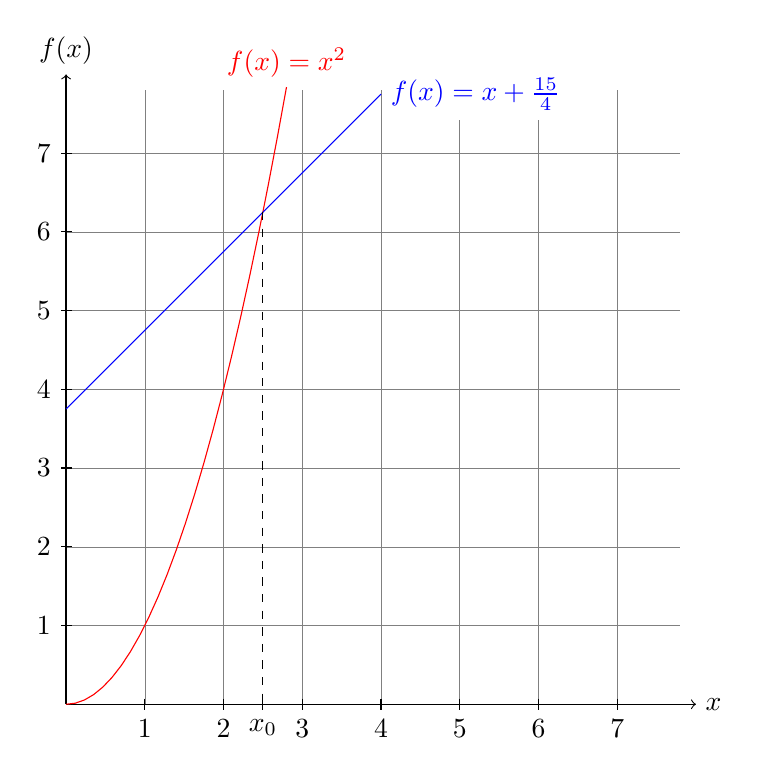
\begin{tikzpicture}
\draw[very thin, gray] (0, 0) grid (7.8,7.8); 
\draw[->] (0,0) -- (8,0) node[right] {$ x$};
\draw[->] (0,0) -- (0, 8) node[above] {$f(x)$};
\draw[red, domain= 0:2.8] plot (\x, {\x^2})
	node[above] {$f(x)=x^2 $};
\draw[blue, domain = 0: 4] plot (\x, {\x + 3.75})
	node[right, fill=white] {$f(x)=x + \frac{15}{4} $};
\foreach \x in {1, 2, 3, 4, 5, 6, 7}
	\draw[xshift= \x cm] (0, 2pt) -- (0, -2pt) node[below, fill=white] {$\x$};
	
\foreach \y in {1, 2, 3, 4, 5, 6, 7}
	\draw[yshift= \y cm] (2pt, 0) -- (-2pt, 0) node[left, fill=white] {$\y$};
\draw[dashed] (2.5, 6.25) -- (2.5,0);
\draw (2.5, 2pt) -- (2.5, -2pt) node[below, fill= white] {$x_0$};
\end{tikzpicture}
\end{center}

Also gilt $(1)$ solange $x\leq x_0$. F\"ur $x_0$ gilt $x_0^2= x_0+\frac{15}{4}$. Wir m\"ussen also $x_0^2-x_0-\frac{15}{4}=0$ l\"osen. Mittels der L\"osungsformel f\"ur quadratische Gleichungen erhalten wir :
$$x_0= \frac{1 \pm \sqrt{1-4(-\frac{15}{4})}}{2}=\frac{1\pm 4}{2}.$$
Da $x_0>0$ folgt $x_0=\frac{5}{2}$.

D.h. f\"ur $a_k\leq x_0^2= \frac{25}{4}$ ist $(1)$ erf\"ullt, die Folge also monoton wachsend. Wir zeigen nun die
\begin{claim}
$$\forall k\in \NN: a_k \leq \frac{25}{4}.$$
\end{claim}
\begin{proof}
Induktion \"uber $k$. Der Induktionsanfang $k=0$ ist einfach $a_0=1<\frac{25}{4}$. Wir nehmen nun an, dass f\"ur ein beliebiges, aber festes $k\in \NN$ gilt $a_k \leq \frac{25}{4}$. Dann berechnen wir:
$$ a_{k+1} = \sqrt{a_k} + \frac{15}{4} 
\leq \sqrt{\frac{25}{4}} + \frac{15}{4}
= \frac{5}{2} + \frac{15}{4} = \frac{25}{4}.$$

Damit haben wir gezeigt, dass $(1)$ immer erf\"ullt ist, d.h. $(a_k)_{k \in \NN}$ ist monoton wachsend. Weiter haben wir gezeigt, dass $0<a_k \leq 25/4$. Also ist $(a_k)_{k\in \NN}$ monoton und beschr\"ankt, also konvergent.
\end{proof}
\item
Wir haben in $i.)$ gezeigt, dass $a:=\lim_{n\rightarrow \infty} a_n\geq 0$. Es gilt:
$$ a =  \lim_{n\rightarrow \infty} a_n= \lim_{n\rightarrow \infty} a_{n+1}
= \lim_{n\rightarrow \infty} \sqrt{a_n} + \frac{15}{4}
\stackrel{\sqrt{\cdot} \text{ stetig}}{=} \sqrt{\lim_{n\rightarrow \infty} a_n} +\frac{15}{4}
= \sqrt{a} + \frac{15}{4}.$$
Wir setzen $x=\sqrt{a}$, dann gilt
$$ x^2= x + \frac{15}{4} \Longrightarrow x^2 -x - \frac{15}{4} = 0 
\stackrel{x= \sqrt{a}\geq 0}{\Longrightarrow} x = \frac{1+\sqrt{1-4\cdot (-\frac{15}{4})}}{2}= \frac{5}{2}.$$
Damit gilt $\lim_{n\rightarrow \infty} a_n = a = x^2=  \frac{25}{4}$.
\end{enumerate}
\end{solution}


\begin{ex}{$(\star)$} Zeigen Sie, dass 
\begin{align*}
\lim_{n \to \infty} \sqrt[n]{n!}= \infty.
\end{align*}
\end{ex}

\begin{solution} Per Definition ist die Exponential gegeben als 
\begin{align*}
e^x = \sum_{n=0}^\infty \frac{x^n}{n!}.
\end{align*}
Es gilt dementsprechend für alle $x \in \mathbb{R}$, dass
\begin{align*}
e^x \geq \frac{x^n}{n!},
\end{align*}
insbesondere also für $x=n \in \mathbb{N}$ auch das
\begin{align*}
e^n \geq \frac{n^n}{n!} \implies n! \geq \left( \frac{n}{e}\right)^n \implies \sqrt[n]{n!} \geq\frac{n}{e} \xrightarrow{n \to \infty} \infty.
\end{align*}
\end{solution}

\begin{ex}{$(\star)$}
\begin{enumerate}[i.)]
\item
Berechnen Sie den folgenden Grenzwert:

$$ \lim_{n \rightarrow \infty} \log \bigg( \Big( \frac{n}{n+1} \Big)^n \bigg).$$


\item
Berechnen Sie alle H\"aufungspunkte der komplexen Folge:

$$ z_n = (n^4 - n^2 + 2)^{1/n} \sin\bigg( \frac{\pi n}{2} \bigg) + i \frac{n + e}{2n + 1}(-1)^n. $$

\item
Zeigen Sie:

$$\lim_{n \rightarrow \infty} \bigg[ (n+1) \cos\bigg( \frac{1}{n+1} \bigg) - n \cos\bigg( \frac{1}{n} \bigg) \bigg]  =1.$$
\end{enumerate}
\end{ex}
\begin{solution}
\begin{enumerate}[i.)]
\item
Wir berechnen:
$$\bigg(\frac{n}{n+1} \bigg)^n 
= \bigg(1-\frac{1}{n+1} \bigg)^n
= \bigg(1-\frac{1}{n+1} \bigg)^{n+1} \cdot \frac{1}{1-\frac{1}{n+1}} \longrightarrow e^{-1}\cdot \frac{1}{1}= e^{-1}, \quad \text{ f\"ur } n \longrightarrow \infty.$$
Aus der Stetigkeit des Logarithmus folgt:
$$ \lim_{n \rightarrow \infty} \log \bigg( \Big( \frac{n}{n+1} \Big)^n \bigg)
= \log \bigg( \lim_{n \rightarrow \infty} \bigg(\frac{n}{n+1} \bigg)^n \bigg)
= \log(e^{-1})= -1.$$

\item
Wir berechnen:
$$ (n^4 - n^2 + 2)^{1/n} = (n^{1/n})^4 \cdot \left(1 - \frac{1}{n^2} + \frac{2}{n^4}\right)^{1/n} 
\longrightarrow 1^4 \cdot 1 = 1, \quad \text{ f\"ur } n\longrightarrow \infty.$$
wobei wir verwendet  haben, dass
\begin{align*}
\left( 1- \frac{1}{n^2} + \frac{2}{n^4}\right)^{1/n} = \exp \left( \frac{1}{n}\log\left[ 1- \frac{1}{n^2}+ \frac{2}{n^4}\right] \right) \xrightarrow{n \to \infty}  \exp(0)=1.
\end{align*}
Desweiteren
$$\frac{n + e}{2n + 1} = \frac{n}{2n+1} + \frac{e}{2n+1} = \frac{1}{2+\frac{1}{n}} + \frac{e}{2n+1} \longrightarrow \frac{1}{2}, \quad \text{ f\"ur } n\longrightarrow \infty.$$

Wir erinnern uns daran, dass gilt:

$$\sin\Big(\frac{\pi n}{2}\Big) = \begin{cases} 0, \qquad \text{f\"ur } n=2k,\ k\in \NN \\ 1, \qquad \text{f\"ur } n=4k+1,\ k\in \NN  \\ -1, \quad \  \text{f\"ur } n=4k+3,\ k\in \NN.\end{cases}$$
Daraus folgt:

$$z_{2k} \longrightarrow \frac{i}{2}, \quad \text{ f\"ur } k \longrightarrow \infty,$$

$$z_{4k+1} \longrightarrow 1-\frac{i}{2}, \quad \text{ f\"ur } k \longrightarrow \infty,$$

$$z_{4k+3} \longrightarrow -1-\frac{i}{2}, \quad \text{ f\"ur } k \longrightarrow \infty,$$
Da diese drei Teilfolgen die ganze Folge \"uberdecken, kann es keine anderen H\"aufungspunkte geben. Damit sind  die H\"aufungspunkte von
$((n^4 - n^2 + 2)^{1/n} \sin\left( \frac{\pi n}{2} \right) + i \frac{n + e}{2n + 1}(-1)^n)_{n\in \NN}$ gerade die Elemente von $\{ \frac{i}{2}, 1-\frac{i}{2}, -1-\frac{i}{2}\}$.
\item
Wir berechnen:
$$(n+1)\cos\Big(\frac{1}{n+1}\Big) -n \cos\Big(\frac{1}{n}\Big)
= \cos\Big(\frac{1}{n+1}\Big) + n\bigg( \cos\Big(\frac{1}{n+1}\Big) - \cos\Big(\frac{1}{n}\Big) \bigg).$$
Wir k\"ummern uns zuerst um den zweiten Term. Der Mittelwertsatz (Satz 8.9) sagt uns, dass ein $\xi \in (\frac{1}{n+1}, \frac{1}{n})$ existiert, sodass:
$$ \cos\Big(\frac{1}{n}\Big) - \cos\Big(\frac{1}{n+1}\Big) 
= -\sin(\xi) \bigg( \frac{1}{n} - \frac{1}{n+1} \bigg) 
= -\sin(\xi) \bigg( \frac{1}{n\cdot(n+1)} \bigg).$$
Also gilt:

$$0\leq \bigg\vert n\bigg( \cos\Big(\frac{1}{n+1}\Big) - \cos\Big(\frac{1}{n}\Big) \bigg) \bigg\vert
= \bigg\vert -\sin(\xi) \cdot \frac{1}{n+1} \bigg\vert 
\leq  \frac{1}{n+1} \longrightarrow 0, \quad \text{ f\"ur } n\longrightarrow \infty.$$
Damit gilt:
$$ \lim_{n \rightarrow \infty} \bigg[ (n+1) \cos\bigg( \frac{1}{n+1} \bigg) - n \cos\bigg( \frac{1}{n} \bigg) \bigg] 
=  \lim_{n \rightarrow \infty} \cos\Big(\frac{1}{n+1}\Big) + \lim_{n \rightarrow \infty}  n\bigg( \cos\Big(\frac{1}{n+1}\Big) - \cos\Big(\frac{1}{n}\Big) \bigg)$$

$$= \cos(0) +0 = 1.$$
\end{enumerate}
\end{solution}

\begin{ex}[$\star$] \
\begin{enumerate}[i)]
\item Es sei $(a_n)_{n \in \mathbb{N}}$ eine reelle Folge derart, dass für ihre Inkremente gilt $|a_{n+1}-a_n| \leq 2^{-n}$. Zeigen Sie, dass $(a_n)_{n \in \mathbb{N}}$ eine Cauchy Folge ist. Bedeutet dies, dass $(a_n)_{n \in \mathbb{N}}$ konvergiert? Warum? 
\item Es sei $(a_n)_{n \in \mathbb{N}}$ eine reelle Folge, welche rekursiv definiert ist mittels: 
\begin{align*}
a_{n+2} = \frac{a_n+a_{n+1}}{2}, \text{ für alle } n \in \mathbb{N}.
\end{align*}
Zeigen Sie, dass dies eine Cauchy Folge ist. Verwenden Sie Teil i). 
\item Berechnen Sie den Grenzwert der Folge aus Teil ii).
\end{enumerate}

\end{ex}


\begin{solution}
\begin{enumerate}[i)]
\item Sei $ \epsilon >0$ fest aber beliebig. Seien $m \leq n$ beliebige natürliche Zahlen, wir setzen $k= n-m \geq 0$ und betrachten den Ausdruck $|a_m-a_{m+k}|$, falls $k=1$ dann wissen wir bereits, dass $|a_m-a_{m+k}| \leq 2^{-m}$. Verwenden wir nun sukzessive die Dreicksungleichung erhalten wir:
\begin{align*}
|a_m-a_{m+k}| &= |(a_m-a_{m+1}) + (a_{m+1}-a_{m+2}) + \dots + (a_{m+k-1}-a_{m+k})| \\
& \leq |a_m-a_{m+1}| + |a_{m+1}-a_{m+2}| + \dots + |a_{m+k-1}-a_{m+k}|\\
& \leq 2^{-m} + 2^{-(m+1)} + \dots + 2^{-(m+k-1)} < \sum_{k=m}^\infty \frac{1}{2^k} = \frac{1}{2^{m-1}}.
\end{align*}
Dies zeigt, dass falls $m,n \geq n_0$ dann haben wir stets die Ungleichung:
\begin{align*}
|a_m-a_n| < \frac{1}{2^{m-1}} \leq \frac{1}{2^{n_0-1}}.
\end{align*}
Wir wählen also $n_0 \in \mathbb{N}$ derart, dass $\frac{1}{2^{n_0-1}} \leq \epsilon$ oder äquivalent $n_0 \geq \log_2 \frac{2}{\epsilon}$. Wir wissen nun, dass $(a_n)_{n \in \mathbb{N}}$ eine Cauchy Folge in $\mathbb{R}$ ist, da $\mathbb{R}$ vollständig ist konvergiert diese Cauchy Folge auch. 

\item Wir bemerken, dass per Definition gilt:
\begin{align*}
a_{n+2}-a_{n+1} = - \frac{a_{n+1}-a_n}{2} = \dots = (-1)^n  \frac{a_2-a_1}{2^n}.
\end{align*}
Folglich gilt für alle $n \in \mathbb{N}$ für die Inkremente:
\begin{align*}
|a_{n+2}-a_{n+1}| \leq |a_2-a_1| 2^{-n}.
\end{align*}
Die Behauptung folgt also dank Teil i). 

\item Es sei $c:= a_2-a_1$. Wir verwenden die Darstellung von $a_n$ als Teleskopische Summe. Wir betrachten also:
\begin{align*}
a_n  &= a_1 + \sum_{k=1}^{n-1} (a_{k+1}-a_k) = a_1 + \sum_{k=1}^{n-1} (-1)^{k-1} \frac{c}{2^{k-1}} \\
& = a_1 + c\sum_{k=0}^{n-2} \left( \frac{-1}{2} \right)^k.
\end{align*}
Lassen wir nun $n \longrightarrow \infty$ streben und verwenden die Geometrische Reihe mit $r= -1/2$ erhalten wir:
\begin{align*}
\lim_{n \rightarrow \infty} a_n = a_1 + c \frac{1}{1-(-1/2)} = a_1 + c \frac{2}{3} = a_1 + \frac{2}{3}(a_2-a_1) = \frac{a_1+2a_2}{3}.
\end{align*}
\end{enumerate}

\end{solution}

\newpage
\section{Reihen}


\begin{ex} Verwenden Sie den Cauchy'schen Verdichtungssatz (Kondensationssatz) um zu zeigen, dass die nachfolgenden Reihen divergieren respektive konvergieren:
\begin{enumerate}[i)]
\item \begin{align*}
\sum_{n=1}^\infty \frac{1}{n}.
\end{align*}
\item \begin{align*}
\sum_{n=1}^\infty \frac{1}{n^2}.
\end{align*}

\item 
\begin{align*}
 \sum_{n=1}^\infty \frac{1}{n^s}, \text{ wobei } s >1. 
\end{align*}

\end{enumerate}

\end{ex}


\begin{solution} Dank dem Cauchy'schen Kondensationssatz wissen wir, dass für eine nicht-negative, nicht-wachsende Folge $f(n)$ von reellen Zahlen gilt $\sum f(n) < \infty \iff \sum 2^n f(2^n)$ also erhalten wir:
\begin{enumerate}[i)]
\item 
\begin{align*}
\sum_{n=1}^\infty 2^n \frac{1}{2^n} = \sum_{n=1}^\infty 1 = \infty.
\end{align*}
da $a_n=1$ keine Nullfolge ist.
\item 
\begin{align*}
\sum_{n=1}^\infty 2^n \frac{1}{(2^n)^2 } = \sum_{n=1}^\infty \frac{1}{2^n}< \infty.
\end{align*}
da geometrische Reihe mit $r= \frac{1}{2}$. 

\item Wir erhalten durch den Cauchy'schen Kondensationssatz die Reihe:
\begin{align*}
 \sum_{n=1}^\infty 2^n \frac{1}{(2^n)^s} = \sum_{n=1}^\infty 2^n \frac{1}{2^{ns}} = \sum_{n=1}^\infty \left(\frac{1}{2^{s-1}}\right)^n < \infty.
\end{align*}
Da $s>1$ und wir erneut eine geometrische Reihe erhalten mit $0 \leq r = 2^{1-s} <1$. 
\end{enumerate}

\end{solution}


\begin{ex}{$(\star)$}
Bestimmen Sie f\"ur die folgenden Reihen, ob sie konvergent und ob sie absolut konvergent sind:

\begin{enumerate}[i.)]
\item
$$\sum_{k\geq 0} \frac{2k}{3k^3+1}.$$

\item
$$\sum_{k\geq 2} \frac{\sin(k\pi/2)}{\log(k)}.$$

\item
$$\sum_{k\geq 1} \frac{2^k k!}{k^k}.$$

\end{enumerate}
\end{ex}
\begin{solution}
\begin{enumerate}[i.)]
\item
Wir berechnen f\"ur $k\geq 1$:

$$ \bigg\vert \frac{2k}{3k^3+1} \bigg\vert = \frac{2k}{3k^3+1}
\leq \frac{2k}{3k^3} \leq \frac{1}{k^2}.$$
Wir wissen, dass $\sum_{k\geq 1} \frac{1}{k^2}$ konvergiert (siehe Seite 43, Anwendung des Cauchy Verdichtungskriterium), folgt mit dem Majorantenkriterium (Prop. 4.8), dass $\sum_{k\geq 0} \frac{2k}{3k^3+1}$ absolut konvergiert.
\item
Es gilt f\"ur $k\in \NN$ gilt $\sin(k\pi)=0$ und $\sin((2k+1)\pi /2)=(-1)^k$. Damit gilt:
$$ \sum_{k\geq 2} \frac{\sin(k\pi/2)}{\log(k)} 
= \sum_{k\geq 1} \frac{\sin((2k+1)\pi/2)}{\log(2k+1)} 
= \sum_{k\geq 1} \frac{(-1)^k}{\log(2k+1)}.$$ 

Da $\frac{1}{\log(2k+1)}>0$ und die Folge $\frac{1}{\log(2k+1)}$ monoton fallend ist mit  $\lim_{k\rightarrow \infty} \frac{1}{\log(2k+1)}=0$, folgt aus dem Leibnizkriterium (Prop. 4.15), dass $\sum_{k\geq 2} \frac{\sin(k\pi/2)}{\log(k)}$ konvergiert.

Wir zeigen, dass $\sum_{k\geq 2} \frac{\sin(k\pi/2)}{\log(k)}$ nicht absolut konvergiert. Dazu brauchen wir die folgende
\begin{claim}
$$\forall j \in \NN: 2j +1 > \log(2j+1).$$
\end{claim}
\begin{proof}
Wir definieren $h: \mathbb{R}_+ \cup \{0\} \to \mathbb{R}$ als $h(x)= 2x+1-\log(2x+1)$. 

Dann gilt $h(0)=1$ und $h'(x)= 2 - \frac{2}{2x+1} >0$.
\end{proof}
Damit erhalten wir:
$$\sum_{k\geq 2} \bigg\vert \frac{\sin(k\pi/2)}{\log(k)} \bigg\vert
= \sum_{k\geq 1} \bigg\vert \frac{(-1)^k}{\log(2k+1)} \bigg\vert 
= \sum_{k\geq 1} \frac{1}{\log(2k+1)}
> \sum_{k\geq 1} \frac{1}{2k+1}.$$
Da die harmonische Reihe divergiert, divergiert $\sum_{k\geq 2} \bigg\vert \frac{\sin(k\pi/2)}{\log(k)} \bigg\vert$, d.h. $\sum_{k\geq 2} \frac{\sin(k\pi/2)}{\log(k)}$ konvergiert nicht absolut.
\item
Sei $a_n=\frac{2^{k}k!}{k^{k}}$. Wir berechnen:
$$ \frac{\vert a_{n+1} \vert}{\vert a_n \vert} 
= \frac{2^{k+1}(k+1)!}{(k+1)^{k+1}} \cdot \frac{k^{k}}{2^{k}k!}
= 2(k+1) \frac{k^k}{(k+1)^{k+1}} = 2 \bigg( \frac{k}{k+1} \bigg)^{k}
= 2 \bigg(1-\frac{1}{k+1}\bigg)^k$$

$$ = 2 \bigg(1-\frac{1}{k+1}\bigg)^{k+1} \frac{1}{1-\frac{1}{k+1}} \longrightarrow 2 e^{-1} = \frac{2}{e}, \quad \text{ f\"ur } k \longrightarrow \infty.$$
Aus dem Quotientenkriterium (Satz 4.12) folgt, dass $\sum_{k\geq 1} \frac{2^k k!}{k^k}$ absolut konvergiert.
\end{enumerate}
\end{solution}


 
\begin{ex}{$(\star)$}
Untersuchen Sie die folgenden Reihen auf Konvergenz und absolute Konvergenz:

\begin{enumerate}[i.)]
\item
$$ \sum_{n\geq 0} (-1)^n \frac{\sqrt{n}}{n+1}.$$

\item
$$ \sum_{n\geq 0} \bigg( \frac{n+5}{3n-2} \bigg)^{3n}.$$

\item
$$ \sum_{n\geq 0} \frac{\exp(3n \log(n))}{(n!)^2}.$$
\end{enumerate}
\end{ex}
\begin{solution}
\begin{enumerate}[i.)]
\item
Wir berechnen f\"ur $n\in \NN$:
$$ \frac{\sqrt{n+1}}{n+2} < \frac{\sqrt{n}}{n+1} 
\Longleftrightarrow \frac{n+1}{(n+2)^2} < \frac{n}{(n+1)^2}$$

$$\Longleftrightarrow n^3+3n^2+3n+1= (n+1)^3 < (n+2)^2 n = n^3+4n^2+4n
\Longleftrightarrow 0 < n^2+n-1.$$
Also ist $(\frac{\sqrt{n}}{n+1})_{n \in \NN}$ monoton fallend. Damit k\"onnen wir das Leibnizkriterium (Prop. 4.15) anwenden, und damit konvergiert $ \sum_{n\geq 0} (-1)^n \frac{\sqrt{n}}{n+1}$.

Wir zeigen, dass $ \sum_{n\geq 0} (-1)^n \frac{\sqrt{n}}{n+1}$ nicht absolut konvergiert. Dazu berechnen wir f\"ur $n \in \NN \setminus \{0\}$:
$$ \bigg\vert (-1)^n \frac{\sqrt{n}}{n+1} \bigg\vert = \frac{\sqrt{n}}{n+1}
\geq \frac{\sqrt{n}}{2n} = \frac{1}{2\sqrt{n}}.$$
Wir wissen (Anwendung des Verdichtungskriteriums, S. 43), dass $\sum_{n\geq 1} \frac{1}{\sqrt{n}}$ divergiert, damit divergiert auch $\sum_{n\geq 1} \frac{1}{2\sqrt{n}}$. Und schliesslich divergiert deswegen 
$\sum_{n\geq 0} \bigg\vert (-1)^n \frac{\sqrt{n}}{n+1} \bigg\vert$. Also ist $\sum_{n\geq 0} \bigg\vert (-1)^n \frac{\sqrt{n}}{n+1} \bigg\vert$ nicht absolut konvergent.
\item
Wir berechnen:
$$ \limsup_{n\rightarrow \infty} \bigg\vert \Big( \frac{n+5}{3n-2} \Big)^{3n} \bigg\vert^{1/n} 
= \limsup_{n\rightarrow \infty} \bigg( \frac{n+5}{3n-2} \bigg)^{3}
= \limsup_{n\rightarrow \infty} \bigg( \frac{1+\frac{5}{n}}{3-\frac{2}{n}} \bigg)^{3} = \bigg(\frac{1}{3} \bigg)^3= \frac{1}{27} <1.$$
Aus dem Wurzelkriterium (Satz 4.11) folgt, dass $\sum_{n\geq 0} \left( \frac{n+5}{3n-2} \right)^{3n}$ absolut konvergiert.
\item
Zuerst bemerken wir, dass $\frac{e^{3n \log(n)}}{(n!)^2}= \frac{n^{3n}}{(n!)^2}$. Es gibt verschiedene Arten, um zu zeigen, dass die Reihe divergiert. Hier sind zwei M\"oglichkeiten:

$\underline{\text{M\"oglichkeit }1: \text{ Nullfolgenkriterium}}$ 

$$\frac{e^{3n \log(n)}}{(n!)^2}= \frac{n^{3n}}{(n!)^2}
= n^n \cdot \bigg(\frac{n^n}{n!}\bigg)^2 
= n^n \cdot \bigg(\frac{n^n}{1 \cdot 2 \cdot \dots \cdots n}\bigg)^2
\geq n^n \cdot 1^2 \geq 1.$$

Damit ist $(\frac{e^{3n \log(n)}}{(n!)^2})_{n \in \NN}$ keine Nullfolge und mit dem Nullfolgenkriterium (Prop. 4.2) folgt, dass $\sum_{n\geq 0} \frac{\exp(3n \log(n))}{(n!)^2}$ divergiert.

$\underline{\text{M\"oglichkeit }2: \text{ Quotientenkriterium}}$

Wir berechnen:
$$ \frac{\bigg(\frac{(n+1)^{3n+3}}{((n+1)!)^2} \bigg)}{\bigg(\frac{n^{3n}}{(n!)^2} \bigg)} 
= \frac{(n+1)^{3n+3}}{n^{3n}} \cdot \frac{(n!)^2}{((n+1)!)^2}
= \frac{(n+1)^{3n}}{n^{3n}} \cdot (n+1)^3 \cdot \frac{1}{(n+1)^2}$$

$$=\underbrace{\bigg(\Big( 1+ \frac{1}{n} \Big)^{n}\bigg)^3}_{\longrightarrow e^3, \text{ f\"ur } n\longrightarrow \infty} \cdot \underbrace{(n+1)}_{\longrightarrow \infty, \text{ f\"ur } n \longrightarrow \infty} \longrightarrow \infty.$$
Aus dem Quotientenkriterium (Satz 4.12) folgt, dass $\sum_{n\geq 0} \frac{\exp(3n \log(n))}{(n!)^2}$ nicht absolut konvergiert. Da alle Terme nichtnegativ sind (dann ist absolute Konvergenz und Konvergenz das gleiche), folgt, dass $\sum_{n\geq 0} \frac{\exp(3n \log(n))}{(k!)^2}$ nicht konvergiert.
\end{enumerate}
\end{solution}


\begin{ex}{$(\star)$}
Berechnen Sie:

$$ \lim_{n \rightarrow \infty} \bigg( \frac{1}{1\cdot 2} + \frac{1}{2\cdot 3} + \frac{1}{3 \cdot 4} + \dots + \frac{1}{(n-1)\cdot n} \bigg).$$
\end{ex}
\begin{solution}
Wir berechnen:
$$ \lim_{n\rightarrow \infty} \sum_{k=1}^{n-1} \frac{1}{k\cdot (k+1)}
= \lim_{n\rightarrow \infty} \sum_{k=1}^{n-1} \left(\frac{1}{k}- \frac{1}{k+1} \right)
= \lim_{n\rightarrow \infty} \bigg(\frac{1}{1}+ \sum_{k=2}^{n-1} \frac{1}{k} - \sum_{k=1}^{n-1} \frac{1}{k+1}\bigg)$$

$$= \lim_{n\rightarrow \infty} \bigg(1+ \sum_{k=2}^{n-1} \frac{1}{k} - \sum_{k=2}^{n-1} \frac{1}{k} -\frac{1}{n}\bigg)
= \lim_{n\rightarrow \infty} \bigg( 1 - \frac{1}{n} \bigg)= 1.$$
\end{solution}

\begin{ex} \ \begin{enumerate}[i)]
\item Existiert ein $s >0$ sodass die nachfolgende Reihe konvergiert?
\begin{align*}
\sum_{n=2}^\infty \frac{1}{\log(n)^s}.
\end{align*}
\item Für welche $s \in \mathbb{R}$ ist die nachfolgende Reihe konvergent?
\begin{align*}
\sum_{n=2}^\infty \frac{1}{n \log^s (n) }.
\end{align*}
\end{enumerate}

\end{ex}

\begin{solution} Wir verwenden das Cauchy Kondensationsverfahren:
\begin{enumerate}[i)]
\item 
\begin{align*}
\sum_{n=2}^\infty \frac{1}{\log(n)^s}< \infty &\iff \sum_{n=2} ^\infty  2^n \frac{1}{\log(2^n)^s}< \infty  \\
& \iff \frac{1}{\log(2)^s} \sum_{n=2}^\infty \frac{2^n}{n^s} < \infty.
\end{align*}
Jedoch konvergiert die letzte Reihe nicht, da $\lim \frac{2^n }{n^s} = \infty$ keine Nullfolge ist für alle $s >0$ (da die exponential Funktion $2^n= \exp(n \log(2))$ schneller wächst als jedes Polynom beliebigen Grades). Also existiert kein $s>0$ sodass die Reihe konvergiert. 
\item
\begin{align*}
\sum_{n=2}^\infty \frac{1}{n \log^s(n)}< \infty &\iff \sum_{n=2}^\infty 2^n \frac{1}{2^n\log^s(2^n)}< \infty \\
& \iff C\sum_{n=2}^\infty \frac{1}{n^s}< \infty, \text{ wobei } C:= \frac{1}{\log^s(2)}.
\end{align*}
Die letzte Reihe konvergiert genau dann wenn $s > 1$ .
\end{enumerate}

\end{solution}


\begin{ex} Zeigen Sie, dass die nachfolgende Reihe konvergiert:
\begin{align*}
 \sum_{k=1}^\infty \frac{2k^2+2k+3}{6k^5+6}.
\end{align*}
\end{ex}

\begin{solution} Für $n \in \mathbb{N}$ betrachten wir die Partialsumme:
\begin{align*}
\sum_{k=1}^n \frac{2k^2 +2k+3}{6k^5+6} = \frac{1}{3} \sum_{k=1}^n \frac{k^2}{k^5+1} + \frac{1}{3} \sum_{k=1}^n \frac{k}{k^5+1} + \frac{1}{2} \sum_{k=1}^n \frac{1}{k^5 +1}. 
\end{align*}
Offensichtlich gilt, dass $k^5+1 \geq k^5$ und somit $\frac{1}{k^5+1} \leq \frac{1}{k^5}$, wir erhalten also die Abschätzung:
\begin{align*}
\sum_{k=1}^n \frac{2k^2 +2k+3}{6k^5+6} \leq \sum_{k=1}^n \frac{1}{k^3} + \sum_{k=1}^n \frac{1}{k^4} + \sum_{k=1}^n \frac{1}{k^5}.
\end{align*}
Lassen wir nun $n \longrightarrow \infty$, dann erkennen wir die konvergenten Reihen,  wir schliessen dass die Reihe konvergiert. 
\\\\
Alternativ können wir auch das Vergleichskriterium verwenden, denn es gilt:
\begin{align*}
\sum_{n=1}^\infty \frac{2n^2 + 2n +3}{6n^5 +6} \sim \sum_{n=1}^\infty \frac{1}{n^3}.
\end{align*}
Wir berechnen hierfür:
\begin{align*}
\lim_{n \rightarrow \infty} \frac{a_n}{b_n} = \lim_{n \rightarrow \infty} \frac{\frac{2n^2 + 2n +3}{6n^5 + 6}}{\frac{1}{n^3}} = \lim_{ n \rightarrow \infty} \frac{n^3(2n^2+2n+3)}{6n^5+6}= \frac{1}{3} \in (0, \infty).
\end{align*}
Wobei wir verwendet haben, dass die dominanten Terme die der Ordnung $n^5$ sind, somit verhält sich die Reihe vergleichbar mit der konvergenten Reihe $\sum \frac{1}{n^3}$. 
\end{solution}


\begin{ex} Zeigen Sie mit Hilfe des Integralkriteriums, dass die folgende Reihe konvergiert:
\begin{align*}
\sum_{n=0}^\infty \frac{1}{n^2+1}.
\end{align*}
\end{ex}


\begin{solution} Wir verwenden das Integralkriterium, d.h. wir betrachten das Integral:
\begin{align*}
\int_0^\infty \frac{1}{x^2 +1}dx = \left. \tan^{-1}(x)\right|_{x=0}^{x=\infty} = \frac{\pi}{2} < \infty.   
\end{align*}
Also konvergiert die Reihe, was zu zeigen war. 
\end{solution}

\begin{ex} Bestimmen Sie, ob die nachfolgende Reihe konvergiert:
\begin{align*}
\sum_{n=0}^\infty ne^{-n^2}.
\end{align*}
\end{ex}

\begin{solution} Wir verwenden den Integraltest und erhalten:
\begin{align*}
\int_0^\infty xe^{-x^2} ~dx = \left. - \frac{1}{2}e^{-x^2}\right|_{x=0}^{x=\infty} = \frac{1}{2} < \infty.
\end{align*}
und folglich konvergiert die Reihe. 
\end{solution}
\newpage


\section{Stetigkeit und Grenzwerte von Funktionen}


\begin{ex}
Zeigen Sie, mit Hilfe der Definition der Stetigkeit, dass die folgende Funktion in $x=1$ stetig ist:
\begin{align*}
h: \begin{cases} \mathbb{R} \setminus \lbrace -1 \rbrace & \longrightarrow \mathbb{R} \\
x & \longmapsto \frac{x^2+x+1}{x+1}. \end{cases}
\end{align*}
\end{ex}


\begin{solution}
Sei $ \epsilon >0$ fest aber beliebig, es sei $\delta$ sodass $0< |x-1| < \delta$, und wir können stets ohne Einschränkung annehmen, dass $\delta < 1$. Wir betrachten den Ausdruck:
\begin{align*}
|h(x)-h(1)| &= \left| \frac{x^2 + x +1}{x+1} - \frac{3}{2} \right| = \left| \frac{2x^2+2x+2-3x-3}{2(x+1)} \right| = \left| \frac{x^2- \frac{1}{2}x- \frac{1}{2}}{x+1} \right| \\
& = \left| \frac{ \left( x + \frac{1}{2}\right) (x-1)}{x+1} \right| = \frac{ \left| x + \frac{1}{2}\right| |x-1|}{|x+1|} < \frac{\left|x + \frac{1}{2} \right|}{|x+1|} \delta.
\end{align*}
Wir wollen also die Terme $x+ \frac{1}{2}$ und $x+1$ kontrollieren. Aus $|x-1| < \delta$ erhalten wir jedoch sofort:
\begin{align*}
\left| x + \frac{1}{2} \right| = \left| x -1 +1 + \frac{1}{2} \right| \leq |x-1| + \frac{3}{2} < \delta + \frac{3}{2}< \frac{5}{2}.
\end{align*}
Es bleibt also nur noch der Ausdruck $|x+1|$. Da wir per Annahme $0 < |x-1| < \delta$ haben,  also $x$ sich beliebig nahe an $1$ befindet, muss sich $x+1$ beliebig Nahe an $2$ befinden, also haben wir:
\begin{align*}
2 -\delta < |x+1| < 2 + \delta.
\end{align*}
und da $\delta <1$ haben wir $|x+1| >1$, also erhalten wir:
\begin{align*}
|h(x)-h(1)| < \frac{\left| x + \frac{1}{2} \right|}{|x+1|} \delta < \frac{5}{2} \delta \overset{!}< \epsilon \iff \delta < \epsilon \frac{2}{5}.
\end{align*} 
Wir wählen also für ein beliebiges $\epsilon >0$ ein $\delta$ derart, dass $0 < \delta < \min \lbrace \frac{2\epsilon}{5},1 \rbrace$ und erhalten dass dann $h$ stetig an der Stelle $x=1$ ist, d.h. wir haben formal gezeigt, dass:
\begin{align*}
\lim_{x \rightarrow 1} h(x) = \lim_{x \rightarrow 1} \frac{x^2 + x+1}{x+1} = \frac{3}{2}.
\end{align*}
\end{solution}


\begin{ex} Sind die 3 nachfolgenden Funktionen Lipschitz-stetig?
\begin{enumerate}[i)]
\item $f:(0, \infty) \longrightarrow \mathbb{R}, \ x \longmapsto \frac{1}{1+x^2}$.
\item $f:[0,1) \longrightarrow \mathbb{R}, \ x \longmapsto \sqrt{x}$ .
\item $f: \mathbb{R} \longrightarrow \mathbb{R}, \ x \longmapsto \sin x$.
\item Finden Sie eine Funktion, welche gleichmässig stetig, aber nicht Lipschitz-stetig ist.
\item Finden Sie eine Funktion, die Lipschitz-stetig, aber nicht differenzierbar ist.

\end{enumerate}

\end{ex}


\begin{solution} 
\begin{enumerate}[i)]

\item \begin{align*}
|f'(x)| = \left| \frac{-2x}{(1+x^2)^2}\right| \leq 1 \implies \text{ Ableitung beschränkt} \implies f \text{ ist Lipschitz-stetig}.
\end{align*}
Wir haben hierbei verwendet, dass gemäss Bernoulli Ungleichung $(1+x^2)^2 \geq 1 + 2x^2$. Desweiteren gilt $1+2x^2 \geq 2x$ weil $1-2x+2x^2 = (1-x)^2 + x^2 \geq 0$. Somit haben wir gezeigt, dass $(1+x^2)^2 \geq 2x$ und folglich die Behauptung. 
\item Für die Ableitung an der Stelle $x=0$ gilt:
\begin{align*}
\lim_{x \rightarrow 0} |f'(x)| = \lim_{x \rightarrow 0} \left| \frac{1}{2 \sqrt{x}} \right| = \infty.
\end{align*}
Also ist die Ableitung an der Stelle $x=0$ unbeschränkt und somit ist $f$ nicht Lipschitz-stetig.
\item Offensichtlich ist die Ableitung durch die $\cos$ Funktion gegeben, welche durch $1$ beschränkt ist und somit ist $f$ Lipschitz-stetig.
\item Wir definieren $f: [0,1] \longrightarrow \mathbb{R}, \ x \longmapsto \sqrt{x}$, dann ist $f$ gleichmässig stetig, aber nicht Lipschitz.
\item Die Betragsfunktion $f: \mathbb{R} \longrightarrow \mathbb{R}, \ x \longmapsto |x|$ ist ein möglicher Kandidat. 
\end{enumerate}


\end{solution}


\begin{ex}
Beweisen Sie, falls $f:\RR \longrightarrow \RR$ stetig und injektiv ist, dann ist $f$ streng monoton.
\end{ex}
\begin{solution}
Wir nehmen an, dass $f$ nicht streng monoton ist. Dann existieren $x_1 < x_2 < x_3$, sodass $f(x_1) \leq f(x_2) \geq f(x_3)$ oder $f(x_1)\geq f(x_2) \leq f(x_3)$. Es gibt nun de facto vier F\"alle, die man untersuchen muss. Man kann es mittels \"Uberlegen auf einen Fall reduzieren. Falls jemandem dieses "ohne Beschr\"ankung der Allgemeinheit" nicht zusagt, so soll er dies in Gedanken durch "man zeigt analog" ersetzen und es zeigen. Dies ist eine gute \"Ubung.\\
Ohne Beschr\"ankung der Allgemeinheit k\"onnen wir annhemen, dass gilt $f(x_1) \leq f(x_2) \geq f(x_3)$. Falls dies nicht der Fall ist, betrachten wir $g: \RR \longrightarrow \RR,~ g(x):=\ -f(x)$. $g$ ist stetig und injektiv, desweiteren ist $g$ genau dann streng monoton, wenn $f$ es ist.\\
Desweiteren k\"onnen wir ohne Beschr\"ankung der Allgemeinheit annehmen, dass $f(x_1) \leq f(x_3)$. Andernfalls betrachten wir $h: \RR \longrightarrow \RR,\ h(x):=f(-x)$.\\
Wir haben nun alles auf den Fall $f(x_1)\leq f(x_3) \leq f(x_2)$ reduziert. Aus dem Zwischenwertsatz (Satz 6.16) folgt, dass es ein $\xi \in (x_1, x_2)$ gibt, sodass $f(x_3)= f(\xi)$, dies steht im Widerspruch, dass $f$ injektiv ist.
\end{solution} 


\begin{ex}{$(\star)$}
Sei $f_n:[0,1] \longrightarrow \RR$ eine Funktionenfolge und $f:[0,1] \longrightarrow \RR$. Entscheiden Sie f\"ur jede der folgenden Aussagen, ob sie wahr oder falsch ist:
\begin{enumerate}[i.)]
\item
Alle $f_n$ sind stetig und $f_n \longrightarrow f$ punktweise $\Longrightarrow$ $f$ ist stetig. 
\item
Alle $f_n$ sind stetig und $f_n \longrightarrow f$ gleichm\"assig $\Longrightarrow$ $f$ ist stetig. 
\item
Alle $f_n$ sind differenzierbar auf $(0,1)$ und $f_n \longrightarrow f$ gleichm\"assig $\Longrightarrow$ $f$ ist differenzierbar auf $(0,1)$. 
\end{enumerate}
\end{ex}
\begin{solution}
\begin{enumerate}[i.)]
\item
Falsch. Gegenbeispiel, $f_n(x)=x^n$ und $f(x)=\begin{cases} 1, \quad x=1 \\ 0,\quad x \neq 1. \end{cases}$
\item
Wahr, Prop. 6.24.
\item
Falsch. Gegenbeispiel, $f_n(x)=\begin{cases} 0, \qquad \qquad \ \ \ x\in [0, 1/2) \\ \frac{n}{2}(x-1/2)^2 , \ x\in [1/2, 1/2+1/n) \\ x-1/2, \quad \quad \ x\in [1/2+1/n, 1], \end{cases}$
und 

$f(x)= \begin{cases} 0,  \qquad \quad \ x\in [0, 1/2) \\ x-1/2 , \ \ x\in [1/2, 1). \end{cases}$
\end{enumerate}
\end{solution}





\begin{ex}
Beweisen Sie, falls $f:\RR \longrightarrow \RR$ stetig und beschr\"ankt ist, dann besitzt $f$ einen Fixpunkt.
\end{ex}
\begin{solution}
Wir definieren $a:=\inf_{x\in \RR} f(x)$ und $b:=\sup_{x\in \RR} f(x)$. Dann gilt $Im(f) \subseteq [a,b]$ und wir k\"onnen $f$ einschr\"anken auf $f:[a,b] \longrightarrow [a,b]$. Da $f$ stetig ist, folgt die Behauptung aus dem Fixpunktsatz.
\end{solution}


\begin{ex}{$(\star)$}
Sei $f:(0,1] \longrightarrow \RR$ gleichm\"assig stetig.
Zeigen Sie: Es existiert ein $c\in \RR$, sodass f\"ur jede Folge $(x_n)_{n\in \NN}$ in $(0,1]$ mit $x_n \longrightarrow 0$ gilt:
$$ f(x_n) \longrightarrow c  \quad \text{ f\"ur } n \longrightarrow \infty.$$
Bemerkung (nicht Teil der Aufgabe): Das bedeutet, dass $\lim_{x \downarrow 0}f(x) = c$.
\end{ex}
\begin{solution}
Sei $(x_n)_{n \in \NN}\subseteq (0,1]$ mit $x_n \longrightarrow 0$. Dann ist $(x_n)_{n \in \NN}$ eine Cauchyfolge (da sie konvergiert). Da $f$ gleichm\"assig stetig ist, ist $(f(x_n))_{n\in \NN}$ ebenfalls eine Cauchyfolge. Da $\RR$ vollst\"andig ist (Satz 3.23), existiert ein $c\in \RR$, sodass $f(x_n) \longrightarrow c$. Sei nun $(y_n)_{n\in \NN}\subseteq (0,1]$, sodass $y_n \longrightarrow 0$. Wir definieren f\"ur $n\in \NN$:
$$z_{2n}:=x_n \quad \text{ und } \quad z_{2n+1}:= y_n.$$
Dann gilt $z_n \longrightarrow 0$. Mit der gleichen Argumentation wie oben, erhalten wir, dass $(f(z_n))_{n\in \NN}$ konvergiert und damit gilt:
$$\lim_{n \rightarrow \infty} f(y_n) = \lim_{n \rightarrow \infty} f(z_{2n+1})
= \lim_{n \rightarrow \infty} f(z_n) = \lim_{n \rightarrow \infty} f(z_{2n})
= \lim_{n \rightarrow \infty} f(x_n) = c.$$
\end{solution}

\begin{ex} Berechnen Sie die folgenden Grenzwerte:
\begin{enumerate}[i)]
\item
$$\lim_{x \rightarrow 0} \frac{\sin(ax)}{x}.$$

\item
$$\lim_{x \rightarrow \infty} \frac{e^x x^5}{x^x}.$$

\item

$$ \lim_{x\rightarrow \infty} \big( x^2+3-\sqrt{x^4+6x^2}  \big)x^2.$$
\end{enumerate}

\end{ex}
\begin{solution}
\begin{enumerate}[i)]
\item
Es gibt mehrere M\"oglichkeiten dies zu zeigen:

$ \underline{\text{M\"oglichkeit } 1: \text{ Potenzreihe:}} $

Es gilt:
$$ \frac{\sin(ax)}{x} = \sum_{j\geq 0} \frac{(-1)^j a^{2j+1}}{(2j+1)!} x^{2j}.$$

Wir berechnen:

$$ \bigg\vert \frac{(-1)^j a^{2j+1}}{(2j+1)!}  \bigg\vert^{\frac{1}{2j}}
= \frac{\vert a \vert^{1+\frac{1}{2j}}}{((2j+1)!)^{\frac{1}{j}}} 
\longrightarrow \vert a \vert \cdot 0= 0, \quad \text{ f\"ur } j\longrightarrow \infty.$$

Die restlichen Koeffizienten von $\sum_{j\geq 0} \frac{(-1)^j a^{2j+1}}{(2j+1)!} z^{2j}$ sind $0$. Damit ist der Konvergenzradius $\rho= \infty$. Wir setzten:
$$ f(z)= \sum_{j\geq 0} \frac{(-1)^j a^{2j+1}}{(2j+1)!} z^{2j} .$$
Nach Satz 7.2 ist $f$ stetig. Damit gilt:

$$ \lim_{x\rightarrow 0} \frac{sin(ax)}{x} = \lim_{x\rightarrow 0} f(x) = f(0)
= \sum_{j\geq 0} \frac{(-1)^j a^{2j+1}}{(2j+1)!} 0^{2j} 
= \frac{(-1)^0 a^{2\cdot 0+1}}{(2\cdot 0+1)!} = a.$$

$ \underline{\text{M\"oglichkeit } 2: \text{L'Hôpital:} } $

Es gilt $\lim_{x\rightarrow 0} \sin(ax)= 0 = \lim_{x\rightarrow 0} x$. Nenner und Z\"ahler sind beide differenzierbar. Mit dem Satz von Hôpital (Satz 8.14) folgt:

$$ \lim_{x\rightarrow 0} \frac{\sin(ax)}{x} = \lim_{x\rightarrow 0} \frac{a \cdot \cos(ax)}{1}
= a \cdot \cos(0)= a.$$
Wobei wir benutzt haben, dass $\cos$ stetig ist und $\cos(0)=1$.
\item
Wir berechnen:
$$ \frac{e^x x^5}{x^x} = e^5 \frac{e^{x-5}}{x^{x-5}}= e^5 \bigg(\frac{e}{x}\bigg)^{x-5}.$$

F\"ur $x\geq 2e$ gilt:

$$0 \leq e^5  \bigg(\frac{e}{x}\bigg)^{x-5} \leq e^5 \bigg(\frac{1}{2}\bigg)^{x-5} \longrightarrow 0,
\quad \text{ f\"ur } x\longrightarrow \infty.$$

Wobei wir benutzt haben, dass $2^{x-5} \longrightarrow \infty$ f\"ur $x\longrightarrow \infty$. Damit gilt $\lim_{x\rightarrow \infty} \frac{e^x x^5}{x^x}= 0$.

\item
Wir berechnen:

$$\big(x^2 + 3 - \sqrt{x^4 + 6x^2}\big)x^2 
= \frac{\big(x^2 + 3 - \sqrt{x^4 + 6x^2}\big)\big(x^2 + 3 + \sqrt{x^4 + 6x^2}\big)x^2}{x^2 + 3 + \sqrt{x^4 + 6x^2}}$$

$$ = \frac{9x^2}{x^2 + 3 + \sqrt{x^4 + 6x^2}} 
= \frac{9}{1 + \frac{3}{x^2} + \sqrt{1 + \frac{6}{x^2}}} \longrightarrow \frac{9}{2}, \quad \text{ f\"ur } x \longrightarrow \infty.$$
Also $\lim_{x\rightarrow \infty} \big(x^2 + 3 - \sqrt{x^4 + 6x^2}\big)x^2 = \frac{9}{2}$.

\end{enumerate}
\end{solution}

 

\begin{ex} Berechnen Sie die folgenden Grenzwerte (möglicherweise $\pm \infty$):
\begin{enumerate}[i)]
\item  \begin{align*}
\lim_{x \rightarrow 0 } x^2 \sin \left( \frac{1}{x} \right) .
\end{align*}
\item \begin{align*}
\lim_{x \rightarrow \infty} \frac{2- \cos x}{x+3}.
\end{align*}
\item \begin{align*}
\lim_{x \rightarrow \infty} \frac{x^2 (2+ \sin^2x)}{x+100}.
\end{align*}
\item \begin{align*}
\lim_{x \rightarrow 0 } x^2 e^{ \sin^3 \left( \frac{1}{x}\right) } .
\end{align*}
\end{enumerate}
\end{ex}

\begin{solution} Wir verwenden in allen Lösungen, dass die trigonometrischen Funktionen von oben durch $1$ und von unten durch $-1$ beschränkt sind. Wir erhalten dann:
\begin{enumerate}[i)]
\item \begin{align*}
0 \longleftarrow -x^2 \leq x^2 \sin \left( \frac{1}{x} \right) \leq x^2 \longrightarrow 0, \text{ falls } x \longrightarrow 0. 
\end{align*}
da $x^2 \geq 0$.
\item Wir haben $-1 \leq \cos (x) \leq 1$ und somit $ 1 \geq - \cos(x) \geq -1 $ also:
\begin{align*}
0 \longleftarrow \frac{1}{x+3} \leq \frac{2- \cos x}{x+3} \leq \frac{3}{x + 3} \longrightarrow 0  \text{ falls } x \longrightarrow \infty.
\end{align*}
\item Es genügt die untere Abschätzung zu betrachten, wir erkennen dass: 
\begin{align*}
\frac{x^2}{x+100} \leq \frac{x^2 (2+ \sin^2 x)}{x+100}.
\end{align*}
und da die untere Schranke gegen unendlich divergiert, muss auch die obere Schranke nach unendlich divergieren. 
\item Da die Exponential Funktion monoton wachsend auf $\mathbb{R}$ ist erhalten wir: 
\begin{align*}
0 \longleftarrow x^2 e^{-1} \leq x^2 \exp \left(  \sin^3 \left( \frac{1}{x} \right) \right) \leq x^2 e^1 \longrightarrow 0, \text{ falls } x \longrightarrow 0.
\end{align*}
\end{enumerate}
\end{solution}


\begin{ex} Berechnen Sie die folgenden Grenzwerte:
\begin{enumerate}[i)]
\item \begin{align*}
 \lim_{x \rightarrow 0^+} \left( \sqrt{x^2 +1} \right)^{ \frac{1}{\sin^2 x}} .
\end{align*}
\item \begin{align*}
\lim_{x \rightarrow 0^+} x^{ \sqrt{x+4}-2}.
\end{align*}
\end{enumerate}

\end{ex}



\begin{solution} Wir verwenden den $e^{\log}$-Trick um diese beiden Aufgaben zu lösen: 
\begin{enumerate}[i)] 
\item 
\begin{align*}
 \lim_{x \rightarrow 0^+} \left( \sqrt{x^2 +1} \right)^{ \frac{1}{\sin^2 x}} = \lim_{ x \rightarrow 0^+} \exp \left( \log \left[ \left( \sqrt{x^2+1}\right)^\frac{1}{\sin^2x} \right] \right) = \lim_{x \rightarrow 0^+} \exp \left( \frac{\log \sqrt{x^2+1}}{\sin^2 x} \right). 
\end{align*}
Da die Exponentialfunktion stetig ist, dürfen wir den Grenzwert mit der $\exp$-Funktion vertauschen (i.e. in ihr Argument hereinziehen). Für den Grenzwert der Funktion im Exponenten erhalten wir mit Hilfe des Satzes von Bernoulli De L'Hopital, dass:
\begin{align*}
\lim_{x \rightarrow 0+} \frac{\log ( \sqrt{x^2+1}}{\sin^2x} = \lim_{x \rightarrow 0^+} \frac{\log(x^2+1)}{2 \sin^2 x} = \lim_{x \rightarrow 0^+} \frac{\frac{2x}{1+x^2}}{4 \sin x \cos x} &= \lim_{x \rightarrow 0^+} \underbrace{\frac{x}{2 \sin x}}_{ \longrightarrow 1/2} \cdot \underbrace{\frac{1}{(1+x^2) \cos x}}_{ \longrightarrow 1}   
\\ & = \frac{1}{2}.
\end{align*}
und somit erhalten wir für den Grenzwert $e^{1/2}$. 

\item 
\begin{align*}
\lim_{x \rightarrow 0^+} x^{ \sqrt{x+4}-2} = \lim_{x \rightarrow 0^+} \exp \left( \log \left( x^{ \sqrt{x+4}-2} \right) \right) = \lim_{x \rightarrow 0^+} \exp \left( (\sqrt{x+4}-2) \log(x) \right). 
\end{align*}
Dann berechnen wir den Grenzwert für die Funktion im Exponenten, erneut mit Hilfe des Satzes von Bernoulli- de L'Hopital:
\begin{align*}
\lim_{ x \rightarrow 0^+} ( \sqrt{4+x}-2) \log(x) & = \lim_{x \rightarrow 0^+} \frac{\log (x)}{\frac{1}{\sqrt{x+4}-2}} = \lim_{x \rightarrow 0^+} \frac{\frac{1}{x}}{\frac{- \frac{1}{2 \sqrt{x+4}}}{(\sqrt{x+4}-2)^2}} \\
&= \lim_{x \rightarrow 0^+} \frac{-2 \cdot \sqrt{x+4} \cdot ( \sqrt{x+4}-2)^2}{x} \\
&=  \lim_{x \rightarrow 0^+} \frac{-4 ( \sqrt{x+4}-2)^2}{x} = \lim_{x \rightarrow 0^+} \frac{-8( \sqrt{x+4}-2) \frac{1}{2 \sqrt{x+4}}}{1} \\
= & \lim_{x \rightarrow 0^+} -8 \underbrace{( \sqrt{x+4}-2)}_{ \longrightarrow 0} \cdot \underbrace{\frac{1}{2 \sqrt{x+4}}}_{ \longrightarrow 1/4}  = 0 .
\end{align*}
Also erhalten wir als Grenzwert $e^0=1$. 
\end{enumerate}
\end{solution}

\begin{ex} Berechnen Sie den folgenden Grenzwert: 
\begin{align*}
\lim_{x \rightarrow 0} \frac{1}{x} \int_0^{\tan x} \log(2+t)dt.
\end{align*}
\begin{solution} Wir haben den Typ $"0/0"$ da $\lim_{x \rightarrow 0} \int_0^{ \tan x} \log (2 +t) dt =0$. Dank dem Hauptsatz der Integralrechnung erhalten wir:
\begin{align*}
\lim_{x \rightarrow 0} \frac{1}{x} \int_0^{\tan x} \log(2+t)dt = \lim_{x \rightarrow 0} \frac{\log(2 + \tan (x)) \cdot \frac{1}{\cos^2 (x)}}{1} = \lim_{x \rightarrow 0} \frac{\log(2 + \tan(x))}{\cos^2 (x)}= \log(2).
\end{align*}
\end{solution}
\end{ex}


\begin{ex} Berechnen Sie den folgenden Grenzwert: Tipp: Verwenden sie einen Fundamentallimes.

\begin{align*}
\lim_{x \rightarrow \infty} \left( \frac{x^2 +2x}{x^2-3x+2}\right)^{ \frac{x^2 +1}{x-3}}.
\end{align*}

\end{ex}


\begin{solution} Wir verwenden den Fundamentallimes $\lim_{x \rightarrow \infty} \left( 1+\frac{1}{x}\right)^x= e$. Wir berechnen also: 
\begin{align*}
\lim_{x \rightarrow \infty} \left( \frac{x^2 +2x}{x^2-3x+2}\right)^{ \frac{x^2 +1}{x-3}} &= \lim_{x \rightarrow \infty} \left( \frac{x^2-3x+2+3x-2+2x}{x^2-3x+2} \right)^\frac{x^2+1}{x-3} \\
&= \lim_{x \rightarrow \infty} \left( 1 + \frac{5x-2}{x^2-3x+2} \right)^\frac{x^2+1}{x-3} \\
&= \lim_{x \rightarrow \infty} \left[ \left( 1 + \frac{1}{\frac{x^2-3x+2}{5x-2}}\right)^\frac{x^2-3x+2}{5x-2}\right]^{ \frac{5x-2}{x^2-3x+2} \frac{x^2+1}{x-3}}.
\end{align*}
Der Ausdruck in den eckigen Klammern [.] konvergiert gemäss Fundamentallimes gegen $e$, also betrachten wir nurnoch den Exponenten, dieser kann jedoch wie folgt vereinfacht werden:
\begin{align*}
\frac{5x-2}{x^2-3x+2} \frac{x^2+1}{x-3} =\frac{5x^3-2x^2+5x-2}{x^3-6x^2+12x-6} \longrightarrow 5 \text{ falls } x \longrightarrow \infty.
\end{align*}
Da die höchst auftretenden Potenzen beide Grad $3$ aufweisen. Wir erhalten also den Grenzwert $e^5$. Als kleine Bemerkung, wir haben verwendet, dass wir eine Funktion der folgenden Form betrachten:
\begin{align*}
\lim_{x \rightarrow \infty} f(x)^{g(x)} = \lim_{x \rightarrow \infty} f(x)^{\lim g(x)}. 
\end{align*}
unter der Annahme, dass die beiden Grenzwerte $\lim f(x)$ und $\lim g(x)$ existieren. Dies gilt gemäss dem $e^{\log}$-Trick. In der Tat wir betrachten:
\begin{align*}
\lim_{x \rightarrow \infty} f(x)^{g(x)} = \lim_{x \rightarrow \infty} \exp \left( \log \left( f(x)^{g(x)} \right) \right) = \lim_{x \rightarrow \infty} \exp \left( g(x) \log(f(x)) \right) = \exp( \lim g(x) \log ( \lim f(x)))  \\
= \lim f(x)^{\lim g(x)}.
\end{align*}
Da sowohl $\exp$ als auch $\log$ stetig sind. 
\end{solution}

\newpage


\section{Potenzreihen}



\begin{ex}
Sei $f:\RR_{> -1} \longrightarrow \RR, \ f(x)=\log(1+x)$.
\begin{enumerate}[i.)]
\item
Bestimmen Sie die Taylorreihe von $f$ um $x_0=0$. Bestimmen Sie den Konvergenzradius $\rho$ dieser Reihe.
\item
Sei $R_2 f(x)$ das Restglied des Taylorpolynoms zweiter Ordnung. Zeigen Sie:
$$ R_2 f(x) \geq 0, \quad \forall \ 0\leq x < \rho. $$
\item
Zeigen Sie f\"ur alle $n>1$:
$$ 1 - \left(1+\frac{1}{n}\right)^{-1}\left(1+ \log\left(1+\frac{1}{n}\right)\right) \leq \frac{1}{2n^2}.$$
\end{enumerate}
\end{ex}
\begin{solution}
\begin{enumerate}[i.)]
\item
Wir zeigen, dass:
$$ \log(1+x)= \sum_{n\geq 1} \frac{(-1)^{n+1}}{n} \ x^n, \quad x\in (-1,1).$$
Zuerst zeigen wir die folgende

\begin{claim}
$$f^{(n)}(x)= \frac{(-1)^{n+1}(n-1)!}{(1+x)^n}, \quad x\in \RR_{>-1} \text{ und } n \in \NN_{\geq 1}.$$
\end{claim}
\begin{proof}
Wir beweisen dies mittels Induktion \"uber $n$. Zuerst zeigen wir die Induktionsverankerung $n=1$:

$$ f'(x) = \frac{1}{1+x} = \frac{(-1)^2(1-1)!}{(1+x)^1}.$$
Wir nehmen nun an, dass die Behauptung f\"ur ein $n\in \NN$ wahr ist. Dann berechnen wir:
$$f^{(n+1)}(x)=  \bigg(\frac{(-1)^{n+1}(n-1)!}{(1+x)^n} \bigg)'
= (-1)^{n+1}(n-1)! \bigg((1+x)^{-n} \bigg)' $$

$$= (-1)^{n+1}(n-1)!(-n) (1+x)^{-n-1}
=\frac{(-1)^{(n+1)+1}((n+1)-1)!}{(1+x)^{n+1}}.$$
\end{proof}
Zus\"atzlich gilt $f^{(0)}(0)= f(0)= \log(1)=0$.
Damit erhalten wir f\"ur die Taylorreihe von $f$ in $x_0=0$ den folgenden Ausdruck:
$$ \sum_{n\geq 0} \frac{f^{(n)}(0)}{n!} \ (x-0)^n
= \sum_{n\geq 1} \frac{(-1)^{n+1}(n-1)!}{n!(1+0)^n} \ x^n 
= \sum_{n\geq 1} \frac{(-1)^{n+1}}{n} \ x^n.$$

Der Konvergenzradius ist gegeben durch:

$$ \rho = \frac{1}{\limsup_{n \rightarrow \infty} (1/n)^{1/n}} = \frac{1}{1}= 1.$$
\item
$\underline{\text{M\"oglichkeit } 1: \text{ Taylorreihe}}$

Das Restglied des Taylorpolynoms zweiter Ordnung ist f\"ur $0\leq x < 1$ gegeben durch:

$$ R_2 f(x) = \sum_{k\geq 3} \frac{(-1)^{k+1}}{k} \ x^k 
=\lim_{n \rightarrow \infty} \sum_{k=3}^{2n} \frac{(-1)^{k+1}}{k} \ x^k \geq 0.$$
Wobei wir benutzt haben, dass:
$$ \sum_{k=3}^{2n} \frac{(-1)^{k+1}}{k} \ x^k 
= \sum_{k=1}^{n-1} \bigg(\frac{(-1)^{(2k+1)+1}}{2k+1} \ x^{2k+1} + \frac{(-1)^{(2k+2)+1}}{2k+2} \ x^{2k+2}\bigg)$$

$$= \sum_{k=1}^{n-1} \bigg(\frac{1}{2k+1} \ x^{2k+1} - \frac{1}{2k+2} \ x^{2k+2}\bigg) 
= \sum_{k=1}^{n-1} \underbrace{\bigg(\frac{1}{2k+1}  - \frac{1}{2k+2} \ x\bigg)}_{\geq 0} \underbrace{ x^{2k+1}}_{\geq 0} \geq 0.$$

$\underline{\text{M\"oglichkeit } 2: \text{ Lagrange Restglied}}$

Alternativ kann man das Restglied von Lagrange (Satz 8.25) verwenden. Es existiert ein $\xi_x \in (0,x)$, sodass:
$$ R_2f(x) = \frac{f^{(3)}(\xi_x)}{3!}x^3 
\stackrel{\text{Behauptung 5}}{=} \frac{2!(-1)^4}{3!(1+\xi_x)^3}x^3
= \frac{1}{3} \cdot \underbrace{\frac{x^3}{(1+\xi_x)^3}}_{\geq 0, \text{ da } x\geq 0 ,\xi_x\geq 0} \geq 0.$$
\item
F\"ur $n>1$ gilt $0<\frac{1}{n} <1$. Wir k\"onnen also schreiben:
$$ \log\bigg(1+\frac{1}{n}\bigg) = f\bigg(\frac{1}{n}\bigg) = \frac{1}{n} - \frac{\left( \frac{1}{n} \right)^2}{2} + R_2 f\bigg(\frac{1}{n}\bigg).$$
Wenn wir diese Identit\"at einsetzen erhalten wir:
$$ 1 - \bigg(1+\frac{1}{n}\bigg)^{-1}\bigg(1+ \log(1+\frac{1}{n})\bigg) 
= 1 - \bigg(1+\frac{1}{n}\bigg)^{-1}\bigg(1+ \frac{1}{n} - \frac{1}{2}\big(\frac{1}{n}\big)^2 + R_2f(\frac{1}{n})\bigg)  $$

$$= \bigg(1+\frac{1}{n}\bigg)^{-1} \frac{1}{2n^2} - 
\underbrace{\bigg(1+\frac{1}{n}\bigg)^{-1}}_{> 0} \underbrace{R_2 f(\frac{1}{n})}_{\geq 0, \text{ wegen } ii.)}  
\leq \bigg(1+\frac{1}{n}\bigg)^{-1} \frac{1}{2n^2} = \frac{n}{n+1} \cdot \frac{1}{2n^2}
\leq \frac{1}{2n^2}.$$
\end{enumerate}
\end{solution}


\begin{ex}
Es sei $f_n : [1, \infty) \longrightarrow \RR, \ f_n(x)= 2n \left( \left(2x \right)^{1/n} -1 \right)$.
\begin{enumerate}[i.)]
\item
Zeigen Sie, dass $(f_n)_{n\in \NN}$ punktweise konvergiert und bestimmen Sie den Grenzwert 
$f:[1, \infty) \longrightarrow \RR$.

Hinweise: Schreiben Sie $\left(2x \right)^{1/n}= \exp\left( 1/n \cdot \log(2x) \right)$.
\item
Zeigen Sie, dass die Konvergenz auf dem Intervall $[1,2]$ gleichm\"assig ist.
\item
Ist die Konvergenz gleichm\"assig auf $[1, \infty)$?
\end{enumerate}
\end{ex}
\begin{solution}
\begin{enumerate}[i.)]
\item
Sei $x \geq 1$. Wir wenden den Satz \"uber die Taylorapproximation mit Langrange'schem Restglied (Satz 8.25) an. Dann existiert ein $\xi_x \in (0, 1/n \log(2x))$, sodass:
$$ \exp\left( \frac{1}{n} \cdot \log(2x) \right) 
= e^0 + e^0\frac{1}{n} \cdot \log(2x) + \frac{e^{\xi_x}}{2} \left( \frac{1}{n} \cdot \log(2x) \right)^2$$

$$= 1 + \frac{1}{n} \cdot \log(2x) + \frac{e^{\xi_x}}{2} \left( \frac{1}{n} \cdot \log(2x) \right)^2.$$

Damit gilt:

$$ 2n \left( \left(2x \right)^{1/n} -1 \right)
= 2n \left( \exp\left( \frac{1}{n} \cdot \log(2x) \right) -1 \right) $$
 
$$= 2\cdot \log(2x) + \frac{e^{\xi_x}}{2n} \log(2x)^2 \longrightarrow 2\log(2x)=:f(x), \quad
 \text{ f\"ur } n\longrightarrow \infty.$$
 
\item
Aus $i.)$ wissen wir, dass es f\"ur jedes $x\in [1,2]$ ein $\xi_x \in (0, 1/n \log(2x))$ gibt, sodass:
$$ \vert f_n(x) - f(x) \vert 
= \bigg\vert 2\cdot \log(2x) + \frac{e^{\xi_x}}{2n} \log(2x)^2 - f(x) \bigg\vert
= \bigg\vert \frac{e^{\xi_x}}{2n} \log(2x)^2 \bigg\vert.$$

Da die Exponentialfunktion und der Logarithmus auf unserem Bereich monoton steigend und nichtnegativ sind, gilt:
$$ \sup_{x\in [1,2]} \vert f_n(x) - f(x) \vert
\leq \frac{e^{\frac{1}{n}\log(4)}}{2n} \log(4)^2
\leq \frac{e^{\log(4)}}{2n} \log(4)^2
= \frac{2 \cdot \log(4)^2}{ n} \longrightarrow 0, \quad \text{ f\"ur } n \longrightarrow \infty.$$
\item
Nein.
 $$\bigg\vert f_n\left(\frac{n^n}{2}\right) - f\left(\frac{n^n}{2}\right) \bigg\vert
 = \vert 2n \left( n - 1 \right) - 2\log(n^n) \vert
 = \vert 2n (n-1 - \log(n)) \vert \longrightarrow \infty, \quad \text{ f\"ur } n \longrightarrow \infty.$$
 Also: 
 $$\sup_{x\in [1, \infty)} \vert f_n(x) - f(x) \vert \longrightarrow \infty, \quad \text{ f\"ur } n \longrightarrow \infty.$$
\end{enumerate}
\end{solution}


\begin{ex}{$(\star)$}
Bestimmen Sie die Konvergenzradien der folgenden Potenzreihen in $z\in \CC$:
\begin{enumerate}[i.)]
\item
$$ \sum_{m\geq 1} \bigg( \sum_{j=1}^m \frac{1}{j} \bigg) z^m.$$
\item
$$ \sum_{k\geq 0} 4k^5 3^k z^{k^2}.$$
\item
$$ \sum_{n\geq 1} \bigg(5- \frac{2}{n} \bigg)^n z^n.$$
\item
$$ \sum_{n\geq 0} i^{n-1}n^n z^n. $$
\item
$$ \sum_{n\geq 0} \frac{2^n}{n!} z^n. $$
\end{enumerate}
\end{ex}
\begin{solution}
\begin{enumerate}[i.)]
\item
$$ 1 = 1^n = \left( n \cdot \frac{1}{n}\right)^{1/n} 
\leq \bigg\vert \sum_{j=1}^{n} \frac{1}{j} \bigg\vert^{1/n}
\leq n^{1/n} \longrightarrow 1, \quad \text{ f\"ur } n \longrightarrow \infty.$$
Damit gilt 
$\lim_{n \rightarrow \infty} \bigg\vert \sum_{j=1}^{n} \frac{1}{j} \bigg\vert^{1/n} =1$ 
und damit:
$$ \rho 
= \frac{1}{\limsup_{n\rightarrow \infty} \bigg\vert \sum_{j=1}^{n} \frac{1}{j} \bigg\vert^{1/n} } 
= \frac{1}{\lim_{n\rightarrow \infty} \bigg\vert \sum_{j=1}^{n} \frac{1}{j} \bigg\vert^{1/n} }
= \frac{1}{1}=1.$$
\item
Die Koeffizienten sind:
$$ a_n = \begin{cases} 0, \qquad \qquad \ n \text{ keine Quadratzahl} \\ 4n^{5/2} 3^{\sqrt{n}}, \quad n \text{ Quadratzahl.}   \end{cases} $$
Wir berechnen:
$$ \vert a_{n^2} \vert^{1/n} =\vert 4n^{5/2}\cdot 3^{\sqrt{n}} \vert^{1/n}
= \underbrace{4^{1/n}}_{\longrightarrow 1} \cdot \underbrace{\left( n^{1/n} \right)^{5/2}}_{\longrightarrow 1^{5/2}=1} \cdot \underbrace{e^{\log(3)/\sqrt{n}}}_{\longrightarrow e^0=1} \longrightarrow 1, \quad \text{ f\"ur } n \longrightarrow \infty.$$
Damit erhalten wir:
$$ \rho = \frac{1}{\limsup_{n \rightarrow \infty} \vert a_n \vert^{1/n}} 
= \frac{1}{\limsup_{n \rightarrow \infty} \vert a_{n^2} \vert^{1/n^2}} 
= \frac{1}{1}= 1.$$
\item
Wir berechnen:
$$ \rho 
= \frac{1}{\limsup_{n \rightarrow \infty} \bigg\vert \left( 5 - \frac{2}{n}\right)^n \bigg\vert^{1/n}}
= \frac{1}{\limsup_{n \rightarrow \infty} \left( 5 - \frac{2}{n}\right)}
= \frac{1}{5}.$$
\item
Wir berechnen:
$$\limsup_{n \rightarrow \infty} \vert i^{n-1}n^n \vert^{1/n}  
\stackrel{\vert i \vert = 1}{=} \limsup_{n \rightarrow \infty} n = \infty.$$
Damit gilt:
$$\rho = 0.$$
\item
Sei $k\in \NN$, dann gilt f\"ur $n\geq k$:
$$ \left( n! \right)^{1/n} 
\geq \left(1\cdot 2 \cdot \cdot 3 \cdot \dots (k-1) \cdot k \cdot \underbrace{k \cdot \dots \cdot k}_{n-k \text{ mal}} \right)^{1/n}
\geq k^{(n-k)/n} = k^{1- k/n}.$$
Damit gilt:
$$ \limsup_{n\rightarrow \infty} (n!)^{1/n} \geq \limsup_{n\rightarrow \infty} k^{1- k/n} = k.$$
Da $k\in \NN$ beliebig war, gilt $\limsup_{n\rightarrow \infty} (n!)^{1/n}= \infty$. Es folgt:
$$ \limsup_{n \rightarrow \infty} \bigg\vert \frac{2^n}{n!} \bigg\vert^{1/n}
= \limsup_{n \rightarrow \infty} \frac{2}{(n!)^{1/n}} =0.$$
Also gilt:
$$ \rho= \infty. $$
\end{enumerate}
\end{solution}


\begin{ex}{$(\star)$}
Entscheiden Sie f\"ur die folgenden Aussagen, ob sie wahr oder falsch sind:
\begin{enumerate}[i.)]
\item
Sei $\rho>0$ der Konvergenzradius von $f(z)= \sum_{n\geq 0} a_n z^n$. Dann ist $f$ auf
$\{ z \in \CC \ : \ \vert z \vert < \rho  \}$ stetig.
\item
Sei $\rho>0$ der Konvergenzradius von $f(z)= \sum_{n\geq 0} a_n z^n$. Dann

$p_m(z)= \sum_{n=0}^m a_n z^n \longrightarrow f(z)$ gleichm\"assig auf $\{ z \in \CC \ : \ \vert z \vert \leq r  \}$ f\"ur alle $r<\rho$.
\end{enumerate}
\end{ex}
\begin{solution}
\begin{enumerate}[i.)]
\item
Wahr, Satz 8.30.
\item
Sei $0\leq r < \rho$. Nach Satz 7.2 konvergiert $\sum_{n\geq 0} \vert a_n \vert \cdot r^n$. Insbesondere gilt $\sum_{n\geq m+1} \vert a_n \vert \cdot r^n \longrightarrow 0$ f\"ur $m\longrightarrow \infty$. Die folgende Rechnung zeigt die gleichm\"assige Konvergenz auf $\{ z \in \CC \ : \ \vert z \vert \leq r  \}$:

$$ \sup_{\vert z \vert \leq r} \vert f(z) - p_m(z) \vert 
= \sup_{\vert z \vert \leq r} \vert \sum_{n\geq m+1} a_n z^n \vert
\leq \sup_{\vert z \vert \leq r}  \sum_{n\geq m+1} \vert a_n \vert \cdot \vert z^n \vert$$

$$= \sum_{n\geq m+1} \vert a_n \vert \cdot r^n \longrightarrow 0, \quad \text{ f\"ur } m \longrightarrow \infty.$$

\end{enumerate}
\end{solution}


\begin{ex} Berechnen Sie den folgenden Grenzwert mit Hilfe der Lagrange'schen Fehlerabschätzung: $$ \lim_{x \rightarrow 0} \bigg( \frac{1}{e^x-1} - \frac{1}{x} \bigg).$$
\end{ex}

\begin{solution}
Aus dem Satz \"uber das Lagrang'sche Restglied (Satz 8.25) wissen wir, dass gilt:
$$ e^x= 1 + x + \frac{x^2}{2} + e^{\xi_x} \cdot \frac{x^3}{6},$$
wobei $\xi_x \in [0,x]$ f\"ur $x>0$ und $\xi_x \in [x,0]$ f\"ur $x<0$. Damit folgt:
$$  \frac{1}{e^x-1} - \frac{1}{x} 
=  \frac{1}{x + \frac{x^2}{2} + e^{\xi_x} \cdot \frac{x^3}{6}} - \frac{1}{x} 
= \frac{1}{x} \bigg( \frac{1}{1 + \frac{x}{2} + e^{\xi_x} \cdot \frac{x^2}{6}} - 1 \bigg)
= \frac{1}{x} \bigg( \frac{-\frac{x}{2} - e^{\xi_x} \cdot \frac{x^2}{6}}{1 + \frac{x}{2} + e^{\xi_x} \cdot \frac{x^2}{6}} \bigg)$$

$$=  \frac{-\frac{1}{2} - e^{\xi_x} \cdot \frac{x}{6}}{1 + \frac{x}{2} + e^{\xi_x} \cdot \frac{x^2}{6}}.$$
Da $\vert \xi_x \vert\leq \vert x \vert$, gilt $\xi_x \longrightarrow 0$ f\"ur $x \longrightarrow 0$. Damit erhalten wir mit der Stetigkeit der Exponentialfunktion:
$$ \lim_{x \rightarrow 0} \bigg( \frac{1}{e^x-1} - \frac{1}{x} \bigg)
=   \lim_{x \rightarrow 0}  \frac{-\frac{1}{2} - e^{\xi_x} \cdot \frac{x}{6}}{1 + \frac{x}{2} + e^{\xi_x} \cdot \frac{x^2}{6}} 
=  \frac{-\frac{1}{2}- e^0\cdot 0}{1+ \frac{0}{2} + e^0\cdot \frac{0^2}{6} }
= -\frac{1}{2}.$$
\end{solution}

\newpage 



\section{Differentialrechnung}

\begin{ex}{$(\star)$}
Sei $f:\RR \longrightarrow \RR$ eine gerade (d.h. $f(x)=f(-x)$ f\"ur alle $x\in \RR$), differenzierbare Funktion. Zeigen Sie, dass $f':\RR \longrightarrow \RR$ eine ungerade Funktion ist, d.h. $f'(-x)=-f'(x).$
\end{ex}
\begin{solution}
Sei $x\in \RR$, dann gilt:
$$ f'(-x) = \lim_{h \rightarrow 0} \frac{f(-x+h)-f(-x)}{h} 
\stackrel{f \text{ gerade}}{=}\lim_{h \rightarrow 0} \frac{f(x-h)-f(x)}{h} 
= \lim_{h \rightarrow 0} \frac{f(x+h)-f(x)}{-h} $$

$$= - \lim_{h \rightarrow 0} \frac{f(x+h)-f(x)}{h} = -f'(x).$$
\end{solution}


\begin{ex}
Beweisen Sie die verallgemeinerte Bernoulli-Ungleichung, welche besagt, dass f\"ur alle $r\geq 1, \ x\geq 0$ gilt:
$$ (1+x)^r\geq 1+rx .$$

Hint: Betrachten Sie die Funktion $h(x)=(1+x)^r - (1+rx).$
\end{ex}
\begin{solution}
Die Behauptung ist \"aquivalent zu der Aussage $h(x)\geq 0$ f\"ur alle $x\geq 0$. Zuerst berechnen wir die Ableitung von $h$:
$$h'(x) = r(1+x)^{r-1} - r = r((1+x)^r -1)\geq 0.$$
Damit ist $h$ monoton steigend. Da $h(0)= 1^r -1=0$, folgt, dass $h(x)\geq 0$ f\"ur alle $x\geq 0$ und damit die Behauptung.
\end{solution}


\begin{ex}{$(\star)$}
Sei $f:\RR \longrightarrow \RR$ definiert durch:
$$ f(x)= \left\{\begin{array}{lr}  x^2 \sin\big( \frac{1}{x} \big), & x\neq 0 \\
0,  & x=0 \end{array}\right. .$$
\begin{enumerate}[i.)]
\item
Zeigen Sie, dass $f$ auf ganz $\RR$ differenzierbar ist und berechnen Sie $f'(x)$ f\"ur alle $x\in \RR$.
\item
Ist $f'$ an der Stelle $x=0$ stetig?
\end{enumerate}
\end{ex}
\begin{solution}
\begin{enumerate}[i.)]
\item
F\"ur $x\neq 0$ erhalten wir mit der Kettenregel (Prop. 8.5) und der Produktregel (Satz 8.3), dass $f$ differenzierbar ist und dass gilt:
$$ f'(x)= (x^2)' \sin\bigg(\frac{1}{x}\bigg) + x^2 \bigg(\sin\bigg(\frac{1}{x}\bigg)\bigg)'
= 2x \sin\bigg(\frac{1}{x}\bigg) + x^2 \bigg(\cos\bigg(\frac{1}{x}\bigg)\bigg) \bigg( \frac{1}{x} \bigg)'$$

$$= 2x \sin\bigg(\frac{1}{x}\bigg) + x^2 \bigg(\cos\bigg(\frac{1}{x^2}\bigg)\bigg) \bigg( \frac{-1}{x^2} \bigg) 
= 2x \sin\bigg(\frac{1}{x}\bigg) - \cos\bigg(\frac{1}{x}\bigg) .$$

F\"ur $x=0$ berechnen wir:
$$0 \leq \bigg\vert \frac{f(h)-f(0)}{h-0} \bigg\vert 
= \bigg\vert \frac{h^2 \sin\big(\frac{1}{x}\big) }{h} \bigg\vert
= \vert h \vert \cdot \bigg\vert \sin\bigg(\frac{1}{x}\bigg) \bigg\vert
\leq \vert h \vert \longrightarrow 0, \quad \text{ f\"ur } h\longrightarrow 0.$$

Damit gilt $f'(0) = \lim_{h\rightarrow 0} \bigg\vert \frac{f(h)-f(0)}{h-0} \bigg\vert =0$.
\item
$f'$ ist stetig in $x=0$, genau dann wenn gilt $\lim_{h\rightarrow 0}f'(h) = f'(0)$, also:
$$ \lim_{h\rightarrow 0} \bigg[ 2h \sin\bigg(\frac{1}{h}\bigg) - \cos\bigg(\frac{1}{h}\bigg) \bigg]=f'(0)=0.$$
Aus der Rechnung von $i.)$ folgt $\lim_{h\rightarrow 0} 2h \sin\left(\frac{1}{h}\right)=0$. Damit ist $f'$ stetig in $x=0$, genau dann wenn $\lim_{h \rightarrow 0} \cos\left(\frac{1}{h}\right)=0$. Dies ist jedoch nicht der Fall. Da:
$$ \cos\left(\frac{1}{\bigg( \frac{1}{2n\pi} \bigg)}\right) = \cos(2n\pi) = 1 \quad \text{ und }  \frac{1}{2n\pi} \longrightarrow 0 \quad \text{ f\"ur } n \longrightarrow \infty.$$
Also ist $f'$ nicht stetig in $x=0$.
\end{enumerate}
\end{solution}

\begin{ex}
Sei $\epsilon>0$. Wir definieren $f_{\epsilon}:\RR \longrightarrow \RR, f_{\epsilon}(x)= \vert x \vert^{1+\epsilon}$.
Zeigen Sie, dass $f_{\epsilon}$ auf ganz $\RR$ differenzierbar ist.
\end{ex}
\begin{solution}
Wir wissen, dass der Absolutbetrag ausserhalb von $x=0$ differenzierbar ist. Auch wissen wir, dass $x\longmapsto x^{1+\epsilon}$ differenzierbar ist (Seite 90). Die Komposition differenzierbarer Funktionen ist differenzierbar (Kettenregel, Prop. 8.5), also ist $f_{\epsilon}$ in $x\neq 0$ differenzierbar. Nun zeigen wir noch, dass $f_{\epsilon}$ in $x=0$ differenzierbar ist

$$\bigg\vert \frac{f_{\epsilon}(h)- f_{\epsilon}(0)}{h-0} \bigg\vert 
= \bigg\vert \frac{\vert h \vert^{1+\epsilon}}{h} \bigg\vert 
= \vert h \vert^{\epsilon} \longrightarrow 0, \quad h \longrightarrow 0.$$
Damit gilt $\lim_{h\rightarrow 0} \frac{f_{\epsilon}(h)-f_{\epsilon}(0)}{h-0}=0$, also ist $f_{\epsilon}$ in $x=0$ differenzierbar (mit $f'_{\epsilon}(0)=0$).
\end{solution}

\begin{ex}
Bestimmen Sie alle Punkte, in denen:
$$f:\RR \longrightarrow \RR,~ f(x)= \left\{\begin{array}{lr}  x^2 , & x\in \QQ \\
0,  & x \in \RR \setminus \QQ \end{array}\right.$$
\begin{enumerate}[i.)]
\item
stetig ist.
\item
differenzierbar ist.
\end{enumerate}
\end{ex}
\begin{solution}
\begin{enumerate}[i.)]
\item
Wir zeigen, dass $f$ nur in $x=0$ stetig ist.

Sei $x\neq 0$. Da sowohl $\QQ$, als auch $\RR \setminus \QQ$ dicht in $\RR$ liegen (Prop. 2.17 und Seite 62), existieren Folgen $(a_n)_{n\in \NN} \subseteq \QQ$ und $(b_n)_{n \in \NN} \subseteq \RR \setminus \QQ$ mit $\lim_{n\rightarrow \infty} a_n = x =\lim_{n \rightarrow \infty} b_n$. Es gilt 
$$ \lim_{n\rightarrow \infty} f(a_n) = \lim_{n \rightarrow \infty} 0 = 0 
\neq x^2 = \lim_{n \rightarrow \infty} b_n^2 = \lim_{n \rightarrow \infty} f(b_n).$$
Damit ist $f$ nicht stetig in $x\neq 0$. Die gleiche Rechnung zeigt, dass $f$ in $x=0$ stetig ist.
\item
Wir zeigen, dass $f$ nur in $x=0$ differenzierbar ist.

Da $f$ nicht stetig ist in $x\neq 0$, ist $f$ auch nicht differenzierbar in $x\neq 0$ (Prop. 8.2). Wir berechnen:
$$ \bigg\vert \frac{f(h)-f(0)}{h-0} \bigg\vert \leq \bigg\vert \frac{h^2}{h} \bigg\vert = \vert h \vert \longrightarrow 0,
\quad h\longrightarrow 0.$$
Damit gilt $\lim_{h\rightarrow 0}\frac{f(h)-f(0)}{h-0}=0$, also ist $f$ in $x=0$ differenzierbar (mit $f'(0)=0$).

Das Ziel dieser Aufgabe war es, daran zu erinneren, dass eine Funktion, die in $x$ differenzierbar ist, nicht in einer ganzen Umgebung von $x$ differenzierbar sein muss. 
\end{enumerate}
\end{solution}


\begin{ex}{$(\star)$}
Berechnen Sie die Ableitungen $f'(x)$ der folgenden Funktionen:
\begin{enumerate}[i.)]
\item
$$ f(x)= \log\bigg(\frac{1 + \sqrt{1-x^2}}{x}\bigg)  \quad \text{ f\"ur } x \in (0,1).$$
\item
$$f(x)= \sqrt{\frac{a+bx}{a-bx}}  \quad \text{ f\"ur } a,b>0,  \text{ f\"ur } x\in \left( \frac{-\alpha}{\beta}, \frac{\alpha}{\beta} \right).$$
\item
$$f(x) = x^{1/3}(1-x)^{2/3}(1+x)^{1/2}  \quad \text{ f\"ur } x\in (0,1).$$
\item
$$f(x)= x^{\sqrt{x}}  \quad \text{ f\"ur } x>0.$$
\item
$$f(x) = \log(\tan(x)^{-1/3}) \quad \text{ f\"ur } x\neq k \frac{\pi}{2},\ k \in \ZZ. $$
\end{enumerate}
\end{ex}
\begin{solution}
\begin{enumerate}[i.)]
\item
$$f'(x) \stackrel{\text{Kettenregel}}{=} \frac{1}{\frac{1 + \sqrt{1-x^2}}{x}} \cdot \bigg(\frac{1 + \sqrt{1-x^2}}{x}\bigg)'$$
$$\stackrel{\text{Quotientenregel}}{=} \frac{x}{1 + \sqrt{1-x^2}} \cdot \frac{(1 + \sqrt{1-x^2})'x - (1 + \sqrt{1-x^2})(x)'}{x^2}$$

$$\stackrel{\text{Kettenregel}}{=} \frac{x}{1 + \sqrt{1-x^2}} \cdot \frac{\frac{-2x}{2 \sqrt{1-x^2}}\cdot x - (1 + \sqrt{1-x^2})}{x^2}
= \frac{x}{1 + \sqrt{1-x^2}} \cdot \frac{\left(\frac{-x^2 - \sqrt{1-x^2} - (\sqrt{1-x^2})^2}{ \sqrt{1-x^2}}\right)}{x^2}$$

$$ =  \frac{x}{1 + \sqrt{1-x^2}} \cdot \frac{\left(\frac{-1 - \sqrt{1-x^2}}{ \sqrt{1-x^2}}\right)}{x^2}
= \frac{x}{1 + \sqrt{1-x^2}} \cdot \frac{-1 - \sqrt{1-x^2}}{x^2 \cdot \sqrt{1-x^2} }
= \frac{-1}{x\cdot \sqrt{1-x^2} }.$$
\item
Man pr\"uft leicht nach, dass: 
$$a-b t >0 \Longleftrightarrow t > -\frac{a}{b} \quad \text{ und }
\quad a+b t >0 \Longleftrightarrow t < \frac{a}{b}.$$
Damit gilt:
$$\frac{a+b t}{a-b t} \geq 0 \Longleftrightarrow t\in \left( -\frac{a}{b}, \frac{a}{b} \right].$$
Wir rechnen:
$$ f'(x)  \stackrel{\text{Kettenregel}}{=} \frac{1}{2\sqrt{\frac{a+bx}{a-bx}}} \cdot \left( \frac{a+bx}{a-bx} \right)' 
\stackrel{\text{Quotientenregel}}{=} \frac{\sqrt{a-bx}}{2\sqrt{a+bx}} \cdot \frac{b\cdot (a-bx) - (a+bx)\cdot(-b)}{(a-bx)^2}$$

$$= \frac{\sqrt{a-bx}}{2\sqrt{a+bx}} \cdot \frac{b\cdot ((a-bx) + (a+bx))}{(a-bx)^2}
= \frac{\sqrt{a-bx}}{\sqrt{a+bx}} \cdot \frac{ab}{(a-bx)^2}.$$
\item
$$f'(x) \stackrel{\text{Produktregel}}{=} \left( x^{1/3} \cdot (1-x)^{2/3} \right)'\cdot (1+x)^{1/2} + x^{1/3} \cdot (1-x)^{2/3} \left( (1+x)^{1/2}\right)'$$

$$\stackrel{\text{Produktregel}}{=} \left( \left(x^{1/3} \right)' \cdot (1-x)^{2/3} + x^{1/3} \left( (1-x)^{2/3} \right)' \right)\cdot (1+x)^{1/2} + x^{1/3} \cdot (1-x)^{2/3} \cdot \frac{1}{2} (1+x)^{-1/2}$$

$$ \stackrel{\text{Kettenregel}}{=} \left( \frac{1}{3} x^{-2/3} \cdot (1-x)^{2/3} - x^{1/3} \cdot \frac{2}{3}(1-x)^{-1/3} \right) \cdot (1+x)^{1/2} + x^{1/3} \cdot (1-x)^{2/3} \cdot \frac{1}{2} (1+x)^{-1/2}$$

$$=\frac{1}{3}x^{-2/3}\cdot (1-x)^{2/3}\cdot (1+x)^{1/2} -\frac{2}{3}x^{1/3}\cdot (1-x)^{-1/3}\cdot (1+x)^{1/2}+ \frac{1}{2} x^{1/3} \cdot (1-x)^{2/3} \cdot (1+x)^{-1/2}$$

$$=\left( \frac{1}{3x^{1/3}} - \frac{2}{3(1-x)^{2/3}} + \frac{1}{2(1+x)^{1/2}} \right)\cdot x^{1/3} \cdot (1-x)^{2/3} \cdot (1+x)^{1/2}.$$
\item
$$f'(x)= \left( e^{\sqrt{x} \cdot\log(x)} \right)'
\stackrel{\text{Produktregel}}{=} \left( \sqrt{x} \cdot\log(x) \right)' \cdot \left( e^{\sqrt{x} \cdot\log(x)} \right)$$

$$\stackrel{Produktregel}{=} \left( (\sqrt{x})' \cdot\log(x) + \sqrt{x} \cdot (\log(x))' \right) \cdot x^{\sqrt{x}}
= \left( \frac{1}{2\sqrt{x}} \cdot\log(x) + \frac{\sqrt{x}}{x} \right) \cdot x^{\sqrt{x}}$$

$$= \frac{1}{\sqrt{x}}\left(\frac{\log(x)}{2} +1\right) x^{\sqrt{x}} 
= \left(\frac{\log(x)}{2} +1\right) x^{\sqrt{x}-1/2} .$$
\item
$$ f'(x) \stackrel{\text{Kettenregel}}{=} \frac{1}{\tan(x)^{-1/3}} \cdot \left( \tan(x)^{-1/3} \right)'
\stackrel{\text{Kettenregel}}{=} \tan(x)^{1/3} \cdot \left( -\frac{1}{3} \right) \tan(x)^{-4/3} \cdot \left( \tan(x) \right)'$$

$$ = -\frac{1}{3} \tan(x)^{-1} \cdot \left(1+ \tan(x)^2 \right)
= -\frac{1}{3} \left( \frac{1}{\tan(x)} + \tan(x) \right).$$
\end{enumerate}
\end{solution}


\begin{ex}{$(\star)$}
Seien $f,g : (a,b) \longrightarrow \RR$ differenzierbare Funktionen.
\begin{enumerate}[i.)]
\item
Zeigen Sie, dass in allen Punkten $x\in (a,b)$ mit $f(x) \neq g(x)$ die Funktion $\max(f,g)$ differenzierbar ist.
\item
Unter welcher Bedingung ist $\max(f,g)$ differenzierbar in einem Punkt $x\in (a,b)$ mit $f(x)=g(x)$.
\end{enumerate}
\end{ex}
\begin{solution}
\begin{enumerate}[i.)]
\item
Sei $x\in (a,b)$.

$\underline{ \text{Fall }1:f(x)-g(x) >0:}$

Da $f,g$ stetig sind, ist $f-g$ ebenfalls stetig (Prop. 6.3) und damit existiert ein $\delta>0$, sodass $(f-g)|_{(x-\epsilon, x+\epsilon)}>0$ gitl. Damit gilt:
$$ \lim_{h\rightarrow 0} \frac{\max(f,g)(x+h) - \max(f,g)(x)}{h}
= \lim_{h\rightarrow 0} \frac{f(x+h) - f(x)}{h} = f'(x).$$

$\underline{ \text{Fall }2:f(x)-g(x) <0:}$
Da $f,g$ stetig sind, ist $f-g$ ebenfalls stetig (Prop. 6.3) und damit existiert ein $\delta>0$, sodass $(f-g)|_{(x-\epsilon, x+\epsilon)}<0$ gilt. Damit gilt:
$$ \lim_{h\rightarrow 0} \frac{\max(f,g)(x+h) - \max(f,g)(x)}{h}
= \lim_{h\rightarrow 0} \frac{g(x+h) - g(x)}{h} = g'(x).$$
\item
\begin{claim}
Sei $x\in (a,b)$:
$$ \max(f,g) \text{ ist differenzierbar in x } \Longleftrightarrow f'(x)=g'(x).$$
\end{claim}
\begin{proof}
$" \Longrightarrow "$ Wir zeigen die Kontraposition. Sei $f'(x)\neq g'(x)$, wir k\"onnen ohne Beschr\"ankung der Allgemeinheit annehmen, dass $f'(x) > g'(x)$ (ansonsten benennen wir unsere Funktionen um). Da $$\lim_{h \rightarrow 0} \frac{(f-g)(x+h)-\overbrace{(f-g)(x)}^{=0}}{h} 
=\lim_{h \rightarrow 0} \frac{(f-g)(x+h)}{h}= f'(x)-g'(x) >0.$$
Damit existiert ein $h_0>0$, sodass f\"ur alle $0<h\leq h_0$:
$$\frac{(f-g)(x+h)}{h} >0 \Longrightarrow f(x+h)>g(x+h)$$
und f\"ur $-h_0\leq h <0$:
$$\frac{(f-g)(x+h)}{h} >0 \Longrightarrow f(x+h)<g(x+h) .$$
Damit gilt:
$$ \lim_{h\downarrow 0} \frac{\max(f,g)(x+h) - \max(f,g)(x)}{h}
= \lim_{h\downarrow 0} \frac{f(x+h) - f(x)}{h} = f'(x) \neq g'(x)$$

$$= \lim_{h\downarrow 0} \frac{g(x+h) - g(x)}{h}
= \lim_{h\uparrow 0} \frac{\max(f,g)(x+h) - \max(f,g)(x)}{h}.$$
Also existiert $\lim_{h\rightarrow 0} \frac{\max(f,g)(x+h) - \max(f,g)(x)}{h}$ nicht. Deswegen ist $\max(f,g)$ in $x$ nicht differenzierbar.

$"\Longleftarrow"$ Sei nun $f'(x)=g'(x)$ f\"ur ein fixes $x\in (a,b)$ und $\epsilon>0$.

Da $\lim_{h \rightarrow 0} \frac{f(x+h)-f(x)}{h}=f'(x)$, existiert ein $\delta_1>0$, sodass f\"ur alle $0 < \vert h \vert < \delta_1$:
$$ \bigg\vert \frac{f(x+h)-f(x)}{h} - f'(x) \bigg\vert < \epsilon.$$
Da $\lim_{h \rightarrow 0} \frac{g(x+h)-g(x)}{h}=g'(x)$, existiert ein $\delta_2>0$, sodass f\"ur alle $0 < \vert h \vert < \delta_2$:
$$ \bigg\vert \frac{g(x+h)-g(x)}{h} - g'(x) \bigg\vert < \epsilon.$$
Damit gilt auch f\"ur alle $0 < \vert h \vert < \delta_2$:
$$ \bigg\vert \frac{g(x+h)-f(x)}{h} -f'(x)\bigg\vert 
\stackrel{f(x)=g(x), \ f'(x)=g'(x)}{=} \bigg\vert \frac{g(x+h)-g(x)}{h} - g'(x) \bigg\vert 
< \epsilon.$$
Sei $\delta=\min\{\delta_1, \delta_2 \}$. Dann gilt f\"ur $0<\vert h \vert <\delta$:
$$\bigg\vert \frac{\max(f,g)(x+h) - \max(f,g)(x)}{h} -f'(x)\bigg\vert 
\stackrel{f(x)=g(x)}{=} \bigg\vert \frac{\max(f,g)(x+h) - f(x)}{h} -f'(x)\bigg\vert$$

$$\leq \max \left\lbrace \underbrace{\bigg\vert \frac{f(x+h) - f(x)}{h} -f'(x)\bigg\vert}_{<\epsilon, \text{ da } \delta\leq \delta_1} \ , \ \underbrace{\bigg\vert \frac{g(x+h) - f(x)}{h} -f'(x)\bigg\vert}_{<\epsilon, \text{ da } \delta \leq \delta_2}  \right\rbrace 
< \epsilon.$$
Damit gilt $\lim_{h \rightarrow 0} \frac{\max(f,g)(x+h) - \max(f,g)(x)}{h}$ konvergiert (gegen $f'(x)$), also ist $\max(f,g)$ in $x$ differenzierbar.
\end{proof}
\end{enumerate}
\end{solution}


\begin{ex}
Seien $n \in \NN_{\geq 1}$, $f\in C^{n}([0,1], \RR)$ und $b\in \RR$. Seien $0\leq x_1< \dots < x_{n+1}\leq 1$ sodass $f(x_i)=b$ f\"ur alle $i\in \{1, \dots , n+1 \}$. Zeigen Sie, es existiert ein $\xi \in (x_1,x_{n+1})$ sodass $f^{(n)}(\xi)=0$.

Hint: Induktion.
\end{ex}
\begin{solution}
Wir beweisen die Behauptung mittels Induktion \"uber $n$.

Die Induktionsverankerung $n=1$ folgt direkt aus dem Mittelwertsatz (Satz 8.9). Wir nehmen an, die Aussage gilt f\"ur ein $n\in \NN_{\geq 1}$. Seien jetzt $0\leq x_1 < \dots < x_{n+2}\leq 1$.
Wir wenden die Induktionsverankerung an, auf die Paare $0\leq x_i < x_{i+1}\leq 1$ f\"ur $i \in \{ 1, \dots , n+1\}$ und erhalten $\xi_{1} < \dots \xi_{n+1}$ mit $x_{i} < \xi_{i} < x_{i+1}$ und 
$f'(\xi_i)=0$. Die Induktionsannahme liefert uns ein $\xi \in (x_1, x_{n+2})$ mit 
$f^{(n+1)}(\xi)=0$.
\end{solution}


\begin{ex}
Sei $K>0$. Wir definieren:
$$ f_n: [-K, K] \longrightarrow \RR, \
f_n(x):= 
\left\{\begin{array}{lr} \frac{n}{2}x^2 + \frac{1}{2n} , & x \in (-\frac{1}{n}, \frac{1}{n}) \\
\vert x \vert,  & \text{sonst}. \end{array}\right. $$
\begin{enumerate}[i.)]
\item
Zeigen Sie, dass $f_n \in C^1([-K,K], \RR)$.
\item
Berechnen Sie den Limes von $(f_n)_{n \in \NN \setminus \{0\}}$ in $(C^0([-K,K], \RR), \Vert \cdot \Vert_{C^0([-K,K], \RR)})$.
\item
Schliessen Sie, dass $(C^1([-K,K], \RR), \Vert \cdot \Vert_{C^0([-K,K], \RR)})$ nicht vollst\"andig ist.
\end{enumerate}
\end{ex}
\begin{solution}
Diese Aufgabe soll daran erinnern, dass der gleichm\"assige Limes von differenzierbaren Funktionen nicht differenzierbar sein muss. In anderen Worten, der Raum der differenzierbaren Funktionen ist nicht vollst\"andig bez\"uglich der Supremumsnorm. \\
Man beachte, dass $(C^1(\RR, \RR), \Vert \cdot \Vert_{C^0(\RR, \RR)})$ kein normierter Vektorraum ist.
\begin{enumerate}[i.)]
\item
$f_n$ ist f\"ur $x \neq \pm 1/n$ offensichtlich stetig. Nun m\"ussen wir die Stetigkeit in $\pm 1/n$ beweisen, dazu benutzen wir Prop. 6.13:

$$ \lim_{x \downarrow \frac{-1}{n}}f_n(x) 
= \lim_{x\downarrow \frac{-1}{n}} \frac{n}{2} x^2 + \frac{1}{2n}
=  \frac{n}{2} \left( \frac{-1}{n} \right)^2 + \frac{1}{2n}
= \frac{1}{n}
= \lim_{x\uparrow \frac{-1}{n}} \vert x \vert
= \lim_{x\uparrow \frac{-1}{n}}f_n(x) .$$

$$ \lim_{x\uparrow \frac{1}{n}}f_n(x) 
= \lim_{x\uparrow \frac{1}{n}} \frac{n}{2}x^2 + \frac{1}{2n}
=  \frac{n}{2} \left( \frac{1}{n} \right)^2 + \frac{1}{2n}
= \frac{1}{n}
= \lim_{x\downarrow \frac{1}{n}} \vert x \vert
= \lim_{x\downarrow \frac{1}{n}}f_n(x).$$

F\"ur die Differenzierbarkeit reicht es analog Serie 11, Aufgabe 2 zu zeigen, dass $\lim_{x\rightarrow a} f_n'(x)$ existiert f\"ur $a\neq \pm 1/n$. Dazu reicht es zu zeigen (Prop. 6.13), dass gilt $\lim_{x\uparrow a} f_n'(x) = \lim_{x\downarrow a}f_n'(x)$. Dies rechnen wir nun nach:

$$ \lim_{x \downarrow \frac{-1}{n}}f'_n(x) 
= \lim_{x\downarrow \frac{-1}{n}} n x
=  -1 
= \lim_{x\uparrow \frac{-1}{n}} -1
= \lim_{x\uparrow \frac{-1}{n}}f'_n(x) .$$

$$ \lim_{x\uparrow \frac{1}{n}}f'_n(x) = \lim_{x\uparrow \frac{1}{n}}nx = 1 = \lim_{x\downarrow \frac{1}{n}} 1
= \lim_{x\downarrow \frac{1}{n}}f'_n(x).$$

Wobei wir benutzt haben, dass der Absolutbetrag differenzierbar ist f\"ur $x\neq 0$ und es gilt:
$$ \vert x \vert' = 
\left\{\begin{array}{lr} 1 , & x>0\\
-1,  & x<0. \end{array}\right. $$
Es bleibt zu zeigen, dass der Limes am Rand existiert (siehe Seite 97). Wir berechnen f\"ur $n\geq 1/K$:
$$ \lim_{x \downarrow -K} f'(x) 
= \lim_{x \downarrow -K} \vert x \vert '
= \lim_{x \downarrow -K} -1
=-1.$$

$$ \lim_{x \uparrow K} f'(x) 
= \lim_{x \uparrow K} \vert x \vert '
= \lim_{x \uparrow K} 1
=1.$$

und f\"ur $n < 1/K$:

$$ \lim_{x \downarrow -K} f'(x) 
= \lim_{x \downarrow -K} n x
=-nK.$$

$$ \lim_{x \uparrow K} f'(x) 
= \lim_{x \uparrow K} n x
=nK.$$
\item
Wir definieren:
$$ f: \RR \longrightarrow \RR, 
f(x)= \ \vert x \vert. $$
Wir zeigen, dass $f_n \longrightarrow f$ bez\"uglich $\Vert \cdot \Vert_{C^0([-K, K], \RR)}$. F\"ur $n\geq 1/K$ gilt:
$$0 \leq \Vert f_n - f \Vert_{C^0([-K,K], \RR)}
= \sup_{x\in [-K,K]} \vert f_n(x) - f(x) \vert
= \sup_{x\in \left(\frac{-1}{n}, \frac{1}{n}\right)} \vert f_n(x) - f(x) \vert$$

$$ \leq  \sup_{x\in \left(\frac{-1}{n}, \frac{1}{n}\right)} \left( \vert f_n(x) \vert + \vert f(x) \vert \right)
\leq \sup_{x\in \left(\frac{-1}{n}, \frac{1}{n}\right)} \vert f_n(x) \vert + \sup_{x\in \left(\frac{-1}{n}, \frac{1}{n}\right)} \vert f(x) \vert$$

$$= \sup_{x\in \left(\frac{-1}{n}, \frac{1}{n}\right)} \Big\vert \frac{n}{2}x^2 + \frac{1}{2n} \Big\vert + \sup_{x\in \left(\frac{-1}{n}, \frac{1}{n}\right)} \vert x  \vert
= \frac{n}{2}\left( \frac{1}{n} \right)^2 + \frac{1}{2n} + \frac{1}{n}
= \frac{2}{n} \longrightarrow 0, \quad \text{ f\"ur } n \longrightarrow \infty.$$
\item
Es gilt $C^1([-K,K], \RR) \subset C^0([-K,K], \RR)$ (Prop. 8.2). Wir wissen aus $ii.)$, dass $(f_n)_{n \in \NN \setminus \{0\}}$ in $(C^0([-K,K], \RR), \Vert \cdot \Vert_{C^0([-K,K], \RR)})$ konvergiert. Damit gilt insbesondere, dass $(f_n)_{n \in \NN \setminus \{0\}}$ eine Cauchyfolge in $(C^0([-K,K], \RR), \Vert \cdot \Vert_{C^0([-K,K], \RR)})$ und damit auch eine Cauchyfolge in $(C^1([-K,K], \RR), \Vert \cdot \Vert_{C^0([-K,K], \RR)})$ ist, da nach $i.)$ $(f_n)_{n \in \NN \setminus \{0\}}\subseteq C^1(\RR, \RR)$. Jedoch gilt $f\notin C^1([-K,K], \RR)$ und damit ist $(C^1([-K,K], \RR), \Vert \cdot \Vert_{C^0([-K,K], \RR)})$ nicht vollst\"andig.
\end{enumerate}
\end{solution}


\begin{ex}{$(\star)$}
\begin{enumerate}[i.)]
\item
Berechnen Sie die Ableitungen der folgenden Funktionen:
\begin{enumerate}
\item
$$ f(x)= \frac{x^2-2x+1}{3x+2},  \quad x\in \RR \setminus \big\{ -\frac{2}{3} \big\} .$$
\item
$$ g(x) = \log((x + \sin(x))^2),  \quad x\in \RR \setminus \{ 0 \}.$$
\item
$$ h(x) = x^{\sin(\sqrt{x})}, \quad x>0.$$
\end{enumerate}
\item
Finden Sie alle lokalen Extrema der Funktion $f(x):=(1+x)\sqrt{\vert x \vert}, \ x\in \RR$.
\end{enumerate}
\end{ex}
\begin{solution}
\begin{enumerate}[i.)]
\item
\begin{enumerate}
\item
$$ f'(x) 
\stackrel{\text{Quotientenregel}}{=} \frac{(x^2-2x+1)' \cdot (3x+2) - (x^2-2x+1)\cdot (3x+2)'}{(3x+2)^2}$$

$$ =\frac{(2x-2) \cdot (3x+2) - (x^2-2x+1)\cdot 3}{(3x+2)^2} 
= \frac{2(x-1)(3x+2) -3(x-1)(x-1)}{(3x+2)^2}$$

$$= \frac{(x-1)(6x+4 -3x+3)}{(3x+2)^2}
= \frac{(x-1)(3x+7)}{(3x+2)^2}.$$
\item
$$g'(x) \stackrel{\text{Kettenregel}}{=} \frac{1}{(x + \sin(x))^2} \cdot \left( (x + \sin(x))^2 \right)'$$

$$\stackrel{\text{Kettenregel}}{=} \frac{1}{(x + \sin(x))^2} \cdot 2( (x + \sin(x))\cdot ( (x + \sin(x))'$$

$$=\frac{1}{(x + \sin(x))^2} \cdot 2( (x + \sin(x))\cdot ( 1+\cos(x))
= \frac{2+2\cos(x)}{ x + \sin(x) }.$$
\item
$$ h'(x) = \left( e^{\sin(\sqrt{x})\cdot \log(x)} \right)' 
\stackrel{\text{Kettenregel}}{=} \left( \sin(\sqrt{x})\cdot \log(x) \right)' \cdot \left( e^{\sin(\sqrt{x})\cdot \log(x)} \right)$$

$$\stackrel{\text{Produktregel}}{=} \left( \sin(\sqrt{x})' \cdot \log(x) + \sin(\sqrt{x}) \cdot \log(x)' \right) \cdot x^{\sin(\sqrt{x})}$$

$$\stackrel{\text{Kettenregel}}{=} \left(\cos(\sqrt{x})\cdot \left( \sqrt{x} \right)' \cdot \log(x) + \frac{\sin(\sqrt{x})}{x}\right) x^{\sin(\sqrt{x})}$$

$$= \left( \frac{\cos(\sqrt{x})}{2\sqrt{x}}\cdot \log(x) + \frac{\sin(\sqrt{x})}{x} \right) \cdot x^{\sin(\sqrt{x})}.$$
\end{enumerate}
\item
Wir unterscheiden in unserer Analysis drei F\"alle:

$\underline{x=0}$:

Zuerst zeigen wir, dass $x=0$ ein lokales Minimum von $f$ ist. Dazu bemerken wir $f(0)=0$. Weiter gilt:
$$ 0<h \Longrightarrow f(h) = \underbrace{(1+h)}_{>0} \underbrace{\sqrt{h}}_{>0} >0$$
und:
$$ -1<h<0 \Longrightarrow f(h) = \underbrace{(1+h)}_{>0} \underbrace{\sqrt{-h}}_{>0} >0.$$

$\underline{x>0}$:

Nun zeigen wir, dass $f$ keine Extrema in $(0, \infty)$ besitzt. F\"ur $x>0$ gilt $f(x)=(1+x)\sqrt{x}$. $f$ ist hier differenzierbar. Es gilt:
$$ 0=f'(x) \stackrel{\text{Produktregel}}{=} \sqrt{x} + \frac{1+x}{2\sqrt{x}} = \frac{3x+1}{2\sqrt{x}}
\Longleftrightarrow 0=  3x + 1 \Longleftrightarrow x= -\frac{1}{3}.$$
Damit besitzt die Gleichung $f'(x)=0$ in $(0, \infty)$ keine L\"osung. Aus Prop. 8.7 folgt, dass $f$ keine Extrema in $(0, \infty)$ besitzt.

$\underline{x<0}$:

F\"ur $x<0$ gilt $f(x)=(1+x)\sqrt{-x}$. $f$ ist hier differenzierbar. Es gilt:
$$ 0=f'(x) \stackrel{\text{Produktregel, Kettenregel}}{=} \sqrt{-x} - \frac{1+x}{2\sqrt{-x}}
=-\frac{3x+1}{2\sqrt{-x}}
\Longleftrightarrow 0= -3x - 1 \Longleftrightarrow x= -\frac{1}{3}.$$

Es gilt $f'(x)>0$ f\"ur $x<-1/3$ und $f'(x)<0$ f\"ur $-1/3 < x < 0$. Aus Prop. 8.13 folgt, dass $x=-1/3$ ein lokales Maximum von $f$ ist. Dies kann man alternativ auch mit Prop. 8.26 beweisen, da:
$$f''(x)
\stackrel{\text{Quotientenregel}}{=} -\frac{6\sqrt{-x} +\frac{(3x+1)}{\sqrt{-x}}}{-4x}
=- \frac{1}{-4x} \cdot \frac{-3x+1}{\sqrt{-x}}$$
und damit:
$$ f''\left( -\frac{1}{3}\right) = \frac{3}{4}\cdot \frac{3}{\sqrt{\frac{1}{3}}}>0.$$

Damit sind $\{ -1/3, 0\}$ alle lokalen Extrema von $f$.
\end{enumerate}
\end{solution}


\begin{ex}
Zeigen Sie, dass die Exponentialabbildung auf $\RR$ konvex ist und zeigen Sie $e^x\geq 1+x$ f\"ur alle $x\in \RR.$
\end{ex}
\begin{solution}
Es gilt $(e^x)''=e^x>0$. Aus Prop. 8.21 folgt, dass die Exponentialabbildung konvex ist. Aus Prop. 8.20 folgt:
$$ e^z \leq \frac{e^y-e^z}{y-z} \leq e^y, \quad \text{ f\"ur } z\leq y. $$
Falls $x>0$, setzen wir $z=0,\ y=x$:
$$ 1= e^0 \leq \frac{e^x - e^0}{x-0} = \frac{e^x-1}{x} \Longrightarrow 1+x \leq e^x.$$
Falls $x<0$, setzen wir $z=x,\ y=0$:
$$ \frac{1-e^x}{-x} = \frac{e^0 -e^x}{-x} \leq e^0 =1  \Longrightarrow 1-e^x \leq -x 
\Longrightarrow 1 +x \leq e^x.$$
\end{solution}


\begin{ex}{$(\star)$}
Zeigen Sie, dass f\"ur alle $x,y \in \RR$ mit $0\leq y<x$ gilt:
$$ ny^{n-1} \leq \frac{x^n - y^n}{x-y} \leq n x^{n-1}, \quad \forall n \in \NN \setminus \{0 \}.$$
\end{ex}
\begin{solution}
F\"ur $y=0$ ist die Aussage trivial. 
Sei $n\in \NN_{\geq 1}$ und $f: \RR_{> 0} \longrightarrow \RR,\ f(x)=x^n$. Es gilt $f^{(2)}(x)= n(n-1)x^{n-2}\geq 0$. Mit Prop. 8.21 ist $f$ konvex und die Aussage folgt aus Prop. 8.20.
\end{solution}


\begin{ex}{$(\star)$}
Entscheiden Sie f\"ur jede der folgenden Aussagen, ob Sie wahr oder falsch ist:
\begin{enumerate}[i.)]
\item
Als Folge in $C^0([0,1], \RR)$ hat $f_n(x)=x^n$ keine gleichmässig konvergente Teilfolge.
\item
Die Funktion $f:\RR \longrightarrow \RR$ definiert durch $f(x)=x^2 \cos(1/x)$ f\"ur $x\neq0$ und $f(0)=0$ ist in $x=0$ differenzierbar.
\item
Sei $f:\RR \longrightarrow \RR$ konvex. Dann ist $f$ auf $\RR$ differenzierbar.
\item
Ist $f:[0,1] \longrightarrow \RR$ gleichm\"assig stetig und auf $(0,1)$ differenzierbar, dann ist $f'$ beschr\"ankt.
\item
Ist $f:[0,1] \longrightarrow \RR$ differenzierbar und es gibt ein $x_0\in (0,1)$ mit $f'(x_0)=0$, so hat $f$ in $x_0$ ein lokales Extremum.
\end{enumerate} 
\end{ex}
\begin{solution}
\begin{enumerate}[i.)]
\item
Wahr. Nehmen wir an, es g\"abe eine gleichm\"assig konvergente Teilfolge $(f_{n_k})_{k\in \NN}$. Diese konvergiert punktweise gegen $f:[0,1]\longrightarrow \RR, f(x) = \begin{cases} 0, \quad x\neq 1 \\ 1, \quad x=1 \end{cases}$. Damit $f_{n_k} \longrightarrow f$ gleichm\"assig. Da die $f_n$ stetig sind, ist $f$ stetig (Prop. 6.24). Dies ist offensichtlich nicht der Fall, also Widerspruch.
\item
Wahr. Es gilt:
$$ 0\leq \bigg\vert \frac{h^2 \cos(\frac{1}{h}) - 0}{h-0} \bigg\vert = \vert h \vert \cdot \big\vert \cos\big(\frac{1}{h}\big) \big\vert \leq \vert h \vert \longrightarrow 0, \qquad \text{f\"ur } h\longrightarrow 0.$$

Damit gilt $\lim_{h\rightarrow 0} \frac{f(h)- f(0)}{h-0}=0$. Also ist $f$ in $x=0$ differenzierbar (mit $f'(0)=0$).
\item
Falsch, der Absolutbetrag ist ein Gegenbeispiel (nicht differenzierbar in $x=0$).
\item
Falsch. Gegenbeispiel $f:[0,1] \longrightarrow \RR, f(x) = \begin{cases} x^2 \cos(\frac{1}{x^3}), \qquad x\neq 0 \\ 0, \qquad \qquad \qquad x=0.\end{cases}$ Man beweist analog zu $ii.)$, dass $f$ stetig ist. Da $[0,1]$ kompakt ist, ist $f$ gleichm\"assig stetig (Satz 6.22). Mittels der Kettenregel (Prop. 8.5) erhalten wir f\"ur $x\in (0,1):$ $f'(x)= 2x \cos(\frac{1}{x^3})+ \frac{1}{x^2} \sin(\frac{1}{x^3})$. Der erste Term ist durch 1 beschr\"ankt und der zweite ist unbeschr\"ankt, also ist $f'$ unbeschr\"ankt.

Ein alternatives Gegenbeispiel ist $g:[0,1]\longrightarrow \RR, \ g(x)=\sqrt{x}$. Wieder folgt aus Satz 6.22, dass $g$ gleichm\"assig stetig ist. Jedoch ist $g'(x)= 1/\sqrt{x}$ unbeschr\"ankt auf $(0,1)$.
\item
Falsch, Gegenbeispiel $f(x)=(x-\frac{1}{2})^3$. $f'\big(\frac{1}{2}\big)= 2\cdot (\frac{1}{2} - \frac{1}{2})^2=0$, aber $x=\frac{1}{2}$ ist weder lokales Maximum, noch Minimum von $f$. Da $f\big(\frac{1}{2}\big)= (\frac{1}{2}-\frac{1}{2})^3=0$. 

F\"ur $x<\frac{1}{2}$ gilt $x-\frac{1}{2}<0$ und damit $f(x)=(x-\frac{1}{2})^3<0$.

F\"ur $x>\frac{1}{2}$ gilt $x-\frac{1}{2}>0$ und damit $f(x)=(x-\frac{1}{2})^3>0$.
\end{enumerate}
\end{solution}


\begin{ex} Sei im folgenden $f:[a,b] \longrightarrow \mathbb{R}$ stetig und auf $(a,b)$ differenzierbar. 
\begin{enumerate}[i)]
\item Verwenden Sie den Satz von Rolle um den Mittelwertsatz zu beweisen.
\item Sei $f'(x)=0$ für alle $x \in (a,b)$, dann gilt: $f(x)$ ist auf $(a,b)$ konstant.
\item Beweisen Sie die folgende Identität 
\begin{align*}
\arctan(x) + \arccos(x) = \frac{\pi}{2}.
\end{align*}
\item Es gilt $f'(x) >0$ für alle $x \in (a,b)$, dann ist $f$ auf $(a,b)$ monoton wachsend. 
\end{enumerate}

\end{ex}


\begin{solution}
\begin{enumerate}[i)]
\item Wir definieren die Hilfsfunktion $g(x):= f(x)-rx$ wobei $r= \frac{f(b)-f(a)}{b-a}$, es gilt dann $g(a)=g(b)$ weil:
\begin{align*}
g(x)=f(x)-rx= f(x)- \frac{f(b)-f(a)}{b-a}x  =  \frac{f(x)(b-a)- (f(b)-f(a))x}{b-a}. 
\end{align*}
Desweiteren erfüllt $g$ die Annahme von Rolle's Theorem, also stetig auf $[a,b]$ und differenzierbar auf $(a,b)$. Also existiert eine $c \in (a,b)$ sodass $g'(c)=0$ gilt. Also:
\begin{align*}
g'(c)=0 = f'(c)-r \iff f'(x) = \frac{f(b)-f(a)}{b-a}.
\end{align*}
\item Seien $x_1,x_2 \in (a,b)$ beliebig. Die Voraussetzungen für den Mittelwertsatz sind erfüllt,  also erhalten wir die Existenz eines $c \in (a,b)$ mit: 
\begin{align*}
\underbrace{f'(c)}_{=0} = \frac{f(x_2)-f(x_1)}{x_2-x_1} \implies f(x_2)=f(x_1).
\end{align*}
Also folgt, dass $f$ auf $(a,b)$ konstant sein muss. 
\item Wir definieren $f(x)= \arctan (x) + \arccos(x)$, wir erhalten dann:
\begin{align*}
f'(x)= \frac{1}{1+x^2 }- \frac{1}{1+x^2}=0.
\end{align*}
Also muss gemäss ii) $f$ konstant auf ganz $\mathbb{R}$ sein. Wir bestimmen die Konstante indem wir $f$ an der Stelle $x=1$ auswerten, wir erhalten dann :
\begin{align*}
f(1)=\arctan(1) + \arccos(1)= \frac{\pi}{4}+ \frac{\pi}{4} = \frac{\pi}{2}.
\end{align*}
Wir erhalten also:
\begin{align*}
\arctan(x) + \arccos(x) = \frac{\pi}{2}.
\end{align*}
\item Wir verwenden erneut den Mittelwertsatz welchen wir in Aufgabe i) bewiesen haben. Wir haben die Existenz eines $c \in (a,b)$ sodass: 
\begin{align*}
\underbrace{f'(c)}_{>0}= \frac{f(x_2)-f(x_1)}{x_2-x_1} \tag{*}.
\end{align*}
Da aber natürlich auch $x_2-x_1>0$ gilt, folgt aus (*), dass $f(x_2)-f(x_1)>0$ also $f(x_2)>f(x_1)$ und somit ist $f$ auf $(a,b)$ monoton wachsend. 
\end{enumerate}
\end{solution}


\newpage
\section{Integrationsrechnung}


\begin{ex} Entscheiden Sie, ob die folgenden Aussagen wahr oder falsch sind, begründen Sie Ihre Antwort: 
\begin{enumerate}[i)]
\item Es sei $f: [a,b] \longrightarrow [0, \infty)$. Dann gilt: $\displaystyle \int_a^bf(x)~dx = 0 \iff f \equiv 0$. 
\item Seien $f,g : [a,b] \longrightarrow \mathbb{R}$ sodass $f \leq g$. Dann gilt: $\displaystyle \int_a^b f(x)~dx \leq \int_a^b g(x) ~dx$.
\item Sei $f: [a,b] \longrightarrow \mathbb{R}$. Dann impliziert $\displaystyle \int_a^b f(x) ~dx >0$, dass $f>0$. 
\item Sei $f:[0, \infty) \longrightarrow \mathbb{R}_+$ monoton fallend mit $\displaystyle \int_0^\infty f(x) ~dx < \infty$. Dann gilt: $\displaystyle \sum_{n=0}^\infty f(n) < \infty$.
\end{enumerate}
\end{ex}


\begin{solution}
\begin{enumerate}[i.)]
\item 
Falsch. Sei z.B. $f(a)=1$ und $f(x)=0 ~~ \forall x \in (a,b]$. Dann ist $f$ nicht konstant null, aber das Integral schon.\\
Bemerkung: Falls $f$ zusätzlich noch stetig ist, wäre die Aussage wahr.

\item
Wahr, Theorem aus Vorlesung, bekannt als die Monotonie des Integrals. 

\item
Falsch. Der negative Teil von $f$ muss nur eine kleinere Fläche haben, als der positive Teil, z.B. $f:[-1,3] \longrightarrow \RR, ~ x \longmapsto x$. Dann gilt
$$\int_{-1}^3 \! f(x) \, \mathrm{d}x ~=~ \frac{1}{2}x^2 \Big|^3_{-1} = ~\frac{9}{2} - \frac{1}{2} ~= 4 >0,$$
und $f(-1)=-1 <0$.

\item
Wahr. Wir benutzen das Integralkriterium für Reihen (Satz 10.5.11). Das liefert uns die Konvergenz der Reihe, sobald wir gezeigt haben, dass $\int_{0}^{\infty} \! g(x) \, \mathrm{d}x < \infty$, wobei $g(x):=f(n)$ falls $x \in [n,n+1)$. Da $f$ monoton fallend ist, gilt $g(x) = f(n) \leq f(n-1) \leq f(x-1) ~ \forall x \in [n,n+1), n\in \NN$. Also gilt $g(x) \leq f(x-1)  ~ \forall x \in [0,\infty)$ und deshalb: $$\int_{0}^{\infty} \! g(x) \, \mathrm{d}x
=\int_{0}^{1} \! g(x) \, \mathrm{d}x + \int_{1}^{\infty} \! g(x) \, \mathrm{d}x
 \leq  a_0 +  \int_{1}^{\infty} \! f(x-1) \, \mathrm{d}x
 = a_0 +  \int_{0}^{\infty} \! f(x) \, \mathrm{d}x <\infty.$$
\end{enumerate}
\end{solution}


\begin{ex} Es sei $t \in \mathbb{R}_>1$. Berechnen Sie die folgenden Integrale:
\begin{enumerate}[i)]
\item \begin{align*}
\int_1^t x^2 ( \ln(x))^2 ~dx.
\end{align*}
\item \begin{align*}
\int_1^3 \frac{2x+3}{x^2+3x+2}~dx.
\end{align*}
\item \begin{align*}
\int_0^t \sin(3x) \cos(5x)~dx .
\end{align*}
\item \begin{align*}
\int_{-2}^3 \frac{56x^7 \cos( \ln (x^8 + 6))}{x^8+6}~dx.
\end{align*}
\item \begin{align*}
\int_0^3 \frac{\cos (x)}{1+\cos(x)}~dx.
\end{align*}
\item \begin{align*}
\int_{-1}^1 \cos(3x) \sqrt{x^4+3x^2 +4} ~dx.
\end{align*}
\item \begin{align*}
\int_0^1 \frac{1}{\sqrt{x+1}+\sqrt{x+2}}~dx.
\end{align*}
\item \begin{align*}
\int_0^1 \ln (1 +x^2 )~dx .
\end{align*}
\item \begin{align*}
\int_2^4 \frac{x^4 +x^3 +x^2+1}{x^2+x-2} ~dx.
\end{align*}
\end{enumerate}
\end{ex}

\begin{solution}
\begin{enumerate}[i.)]
\item
Wir benutzen zwei mal partielle Integration (PI):
\begin{equation}
\begin{aligned}
\int_1^t \! x^2 \left( \ln(x) \right) ^2 \, \mathrm{d}x 
& \stackrel{PI}{=} \frac{1}{3}x^3\left( \ln(x) \right) ^2 {\Bigg|} ^t_1 - \int_1^t \! \frac{1}{3}x^3 ~ 2 \frac{1}{x}~ \ln(x) \, \mathrm{d}x\\
&=\frac{1}{3}t^3\left( \ln(t) \right) ^2-\int_1^t \! \frac{2}{3}x^2 ~ \ln(x) \, \mathrm{d}x\\
& \stackrel{PI}{=}\frac{1}{3}t^3\left( \ln(t) \right) ^2 - \left( \frac{2}{9} x^3 \ln(x){\Bigg|} ^t_1 - \int_1^t \! \frac{2}{9}x^3 ~ \frac{1}{x} \, \mathrm{d}x
\right)\\
&= \frac{1}{3}t^3\left( \ln(t) \right) ^2 - \frac{2}{9} t^3 \ln(t) + \int_1^t \! \frac{2}{9}x^2 \, \mathrm{d}x\\
&= \frac{1}{3}t^3\left( \ln(t) \right) ^2 - \frac{2}{9} t^3 \ln(t) + \frac{2}{27}x^3{\Bigg|} ^t_1\\
&= \frac{1}{3}t^3\left( \ln(t) \right) ^2 - \frac{2}{9} t^3 \ln(t) + \frac{2}{27}t^3 -\frac{2}{27}.
\notag
\end{aligned}
\end{equation}

\item
\underline{1. Möglichkeit: Partialbruchzerlegung}:\\
Wir bemerken, dass $x^2+3x+2= (x+2)(x+1)$ und suchen nun $a,b \in \RR$ mit:
$$ \frac{2x+3}{x^2+3x+2} = \frac{a}{x+2} + \frac{b}{x+1} = \frac{a(x+1) +b(x+2)}{x^2+3x+2} = \frac{x(a+b) +(a+2b)}{x^2+3x+2}.$$
Wir vergleichen die Koeffizienten von den Zählern vom ersten und dem letzten Bruch und kommen auf das Gleichungssystem
$\begin{cases} 2=a+b \\ 3=a+2b \end{cases}$.\\
Das hat die Lösung $a=1=b$ und wir schliessen daraus, dass:
\begin{equation}
\begin{aligned}
\int_1^3 \! \frac{2x+3}{x^2+3x+2} \, \mathrm{d}x 
&= \int_1^3 \! \frac{1}{x+2} + \frac{1}{x+1} \, \mathrm{d}x = \Big( \ln(x+2) + \ln(x+1) \Big){\Bigg|} ^3_1\\
&= \ln\big((x+2)(x+1)\big){\Bigg|} ^3_1
= \ln(20)-\ln(6)= \ln\left(\frac{20}{6}\right)= \ln\left(\frac{10}{3}\right).
\notag
\end{aligned}
\end{equation}
\underline{2. Möglichkeit: Substitution}:\\
Sei $u(x):= x^2+3x+2$. Dann gilt $u'(x)= 2x+3$, was genau dem Zähler entspricht. Wir rechnen also:
$$\int_1^3 \! \frac{2x+3}{x^2+3x+2} \, \mathrm{d}x 
= \int_1^3 \! \frac{u'(x)}{u(x)} \, \mathrm{d}x 
= \int_{u(1)}^{u(3)} \! \frac{1}{u} \, \mathrm{d}u
= \ln(u) {\Bigg|} ^{3^2+3\cdot3+2}_{1^2 +3\cdot1+2}
= \ln(20)-\ln(6)=  \ln\left(\frac{10}{3}\right).$$

\item
Wir benutzen zwei mal partielle Integration (PI) um wieder zum ursprünglichen Integral zu kommen:
\begin{flalign}
& \int_0^t \! \sin(3x)\cos(5x) \, \mathrm{d}x &
\notag
\end{flalign}
\begin{equation}
\begin{aligned}
&\stackrel{PI}{=} -\frac{1}{3}\cos(3x)\cos(5x) \Big|^t_0 -  \int_0^t \! \left(-\frac{1}{3}\cos(3x)\right)\left(-5\sin(5x)\right) \, \mathrm{d}x \\
&= -\frac{1}{3}\cos(3t)\cos(5t) +\frac{1}{3} -  \int_0^t  \frac{5}{3}\cos(3x)\sin(5x) \,\mathrm{d}x \\
&\stackrel{PI}{=} -\frac{1}{3}\cos(3t)\cos(5t) +\frac{1}{3} - \frac{5}{3}\left(\frac{1}{3}\sin(3x)\sin(5x) \Big|^t_0 - \int_0^t  \frac{1}{3}\sin(3x)\cdot 5\cos(5x) \,\mathrm{d}x \right)\\
&= -\frac{1}{3}\cos(3t)\cos(5t) +\frac{1}{3} - \frac{5}{9}\sin(3t)\sin(5t) + \frac{25}{9}\int_0^t  \sin(3x)\cos(5x) \,\mathrm{d}x. 
\notag
\end{aligned}
\end{equation}
Nun subtrahieren wir den letzten Term und bekommen:
$$ (1-\frac{25}{9}) \int_0^t \! \sin(3x)\cos(5x) \, \mathrm{d}x = -\frac{1}{3}\cos(3t)\cos(5t) +\frac{1}{3} - \frac{5}{9}\sin(3t)\sin(5t).$$
Teilen wir durch $-\frac{16}{9}$, liefert uns das das gewünschte Resultat:
$$\int_0^t \! \sin(3x)\cos(5x) \, \mathrm{d}x =
\frac{3}{16}\cos(3t)\cos(5t) -\frac{3}{16} + \frac{5}{16}\sin(3t)\sin(5t).$$

\item
Wir benutzen die Substitutionsmethode mit $u(x):= \ln(x^8+6)$. Dann gilt $u'(x)=\frac{8x^7}{x^8+6}$ und wir erkennnen, dass:
\begin{equation}
\begin{aligned}
\int_{-2}^3 \! \frac{56x^7\cos(\ln(x^8+6))}{x^8+6} \, \mathrm{d}x
&= \int_{-2}^3 \! 7u'(x)\cos(u(x)) \, \mathrm{d}x 
= 7 \int_{u(-2)}^{u(3)} \! \cos(u) \, \mathrm{d}u \\
&=7\sin(u) \Big|^{\ln(6567)}_{\ln(262)}
= 7\sin(\ln 6567)-7\sin(\ln 262).
\notag
\end{aligned}
\end{equation}

\item
Wir benutzen den Additionssatz und $\sin^2(x)+\cos^2(x)=1$ für:
$$1+\cos(x) = 1+\cos\left(\frac{x}{2}+\frac{x}{2}\right) = 1+\cos^2\left(\frac{x}{2} \right) - \sin^2\left(\frac{x}{2} \right)= \cos^2\left(\frac{x}{2} \right)+\cos^2\left(\frac{x}{2} \right) = 2\cos^2\left(\frac{x}{2} \right),$$
und deshalb ist:
$$\left(\tan\left(\frac{x}{2} \right) \right)' = \frac{1/2}{\cos^2\left(\frac{x}{2} \right)} = \frac{1}{1+\cos(x)}.$$
Wir berechnen nun das Integral:
\begin{equation}
\begin{aligned}
\int_0^3 \! \frac{\cos(x)}{1+\cos(x)} \, \mathrm{d}x 
&=\int_0^3 \! \frac{1+\cos(x)-1}{1+\cos(x)} \, \mathrm{d}x 
= \int_0^3 \! 1-\frac{1}{1+\cos(x)} \, \mathrm{d}x\\
&= \left( x-\tan\left(\frac{x}{2}\right) \right)\Big|^3_0
=3-\tan\left(\frac{3}{2}\right). 
\notag
\end{aligned}
\end{equation}

\item
Die Funktion ist als Produkt einer ungeraden Funktion mit einer geraden Funktion ungerade, nämlich sei $f(x):={\cos(3x)}\sqrt{x^4+3x^2+4}$. Dann gilt für $x \in [-1,1]$:
$$f(-x)={\cos(-3x)}\sqrt{(-x)^4+3(-x)^2+4} = -{\cos(3x)}\sqrt{x^4+3x^2+4} = -f(x).$$
Dann gilt:
\begin{equation}
\begin{aligned}
\int_{-1}^1 \! {\cos(3x)}\sqrt{x^4+3x^2+4} \, \mathrm{d}x
 &= \int_{-1}^1 \! f(x) \, \mathrm{d}x 
= \int_{-1}^0 \! f(x) \, \mathrm{d}x+\int_{0}^1 \! f(x) \, \mathrm{d}x\\
&=\int_{0}^1 \! f(-x) \, \mathrm{d}x+\int_{0}^1 \! f(x) \, \mathrm{d}x\\
&=-\int_{0}^1 \! f(x) \, \mathrm{d}x+\int_{0}^1 \! f(x) \, \mathrm{d}x = 0.
\notag
\end{aligned}
\end{equation}

\item
Wir benutzen die dritte binomische Formel:
\begin{equation}
\begin{aligned}
\int_0^1 \! \frac{1}{\sqrt{x+1}+ \sqrt{x+2}} \, \mathrm{d}x
&= \int_0^1 \! \frac{1}{\sqrt{x+1}+ \sqrt{x+2}}\frac{\sqrt{x+1}- \sqrt{x+2}}{\sqrt{x+1}- \sqrt{x+2}} \, \mathrm{d}x\\[.3cm]
&= \int_0^1 \! \frac{\sqrt{x+1}- \sqrt{x+2}}{x+1- (x+2)} \, \mathrm{d}x\\[.1cm]
&=\int_0^1 \! -(\sqrt{x+1}- \sqrt{x+2})\, \mathrm{d}x\\
&= \bigg( -\frac{2}{3\sqrt{x+1}^3} + \frac{2}{3\sqrt{x+2}^3} \bigg) \Bigg|^1_0\\
&= \frac{2}{3}- \frac{8\sqrt{2}}{2}+2\sqrt{3}. 
\notag
\end{aligned}
\end{equation}

\item
Wir integrieren partiell:
\begin{equation}
\begin{aligned}
\int_{0}^1 \! \ln(1+x^2) \cdot 1\, \mathrm{d}x &= \ln(1+x^2)x \Big|^1_0 - \int_{0}^1 \! \frac{2x}{1+x^2}\cdot x~ \, \mathrm{d}x \\
&= \ln(2) - \int_{0}^1 \! \frac{2(x^2+1)-2}{1+x^2} \, \mathrm{d}x\\
&= \ln(2) - \int_{0}^1 \!2- \frac{2}{1+x^2} \, \mathrm{d}x\\
&= \ln(2) - \big( 2x-2\arctan(x) \big) \Big|^1_0\\
&= \ln(2)-2+\frac{\pi}{2} .
\notag
\end{aligned}
\end{equation}

\item Da der Grad des Zählers grösser ist als der Grad des Nenners müssen wir zuerst eine Polynomdivision durchführen, wir erhalten: 
\begin{align*}
\frac{x^4+x^3+x^2+1}{x^2+x-2} = x^2 + 3 + \frac{-3x+7}{x^2+x-2}.
\end{align*}
Weil:  \\ \\ 
\polylongdiv[style=C]{x^4+x^3+x^2+1}{x^2+x-2}.
\\
Für den zweiten Term verwenden wir Partialbruch-Zerlegunng, wir verwenden den Ansatz:
\begin{align*}
\frac{-3x+7}{x^2+x-2}= \frac{-3x+7}{(x+2)(x-1)} = \frac{A}{x+2} + \frac{B}{x-1}.
\end{align*}
Wir erhalten also nach Multiplikation mit $(x+2)(x-1)$ die Aussage:
\begin{align*}
A(x-1)+B(x+2)=-3x+7.
\end{align*}
Setzen wir $x=1$ erhalten wir $B= \frac{4}{3}$ und für $x=-2$ erhalten wir $A= - \frac{13}{3}$. 
Somit haben wir gezeigt, dass:
\begin{align*}
\frac{x^4+x^3+x^2+1}{x^2+x-2}= x^2 + 3 - \frac{13}{3} \frac{1}{x+2} + \frac{4}{3} \frac{1}{x-1}.
\end{align*}
Nun liefert die Integration über die Grenzen schliesslich:
\begin{align*}
\int_2^4  \frac{x^4+x^3+x^2+1}{x^2+x-2}~dx &= \left. \frac{x^3}{3} + 3x - \frac{13}{3} \ln (x+2)+ \frac{4}{3} \ln ( x-1) \right|_{x=2}^{x=4} \\ 
&= \frac{74}{3} + \ln \left( \frac{16 \sqrt[3]{2}}{27} \right).
\end{align*}
\end{enumerate}
\end{solution}


\end{document}
